\setcounter{subsection}{0} 
\part{Appendix}
\subsection{Signal sample analysis scripts}
The scripts related to decay files, generation files and steering files are presented in the appendix A. Only the key highlights of the complete macros are reported, in order to ensure a smoother reading.

\subsection{The decay file and the generation steering file}
Monte Carlo (MC) truth is widely used in High Energy Physics (HEP) experiments. It allows the generation of datasets that follow a specific physical process, propagating particles through the detector and mimicking its behaviour layer by layer. These datasets are processed like real data during the reconstruction phase, with the advantage that the true information from the MC generator is known. The more realistic the MC simulation, the better the understanding of the real dataset.
$\\$
The production of a MC sample is divided in three main steps: 
\begin{itemize}
\item The generation of the MC particles with a generator 
\item The simulation of the detector structure and response to a particle (propagation)
\item The reconstruction of tracks, cluster etc.
\end{itemize}
$\\$
The decay file represents the first step to generate events specifying the decay channels of interest. It is the script in which the decay channel of a specific particle is explicitly set to a desired mode. It allows to impose several constraints on particle decay modes, in order to study a specific detector response or the kinematics of a given particle. This is called in jargon "generating signal MC events". The related file has \emph{.dec} extension.
$\\$
An example from section 3 is explained in Fig.~\ref{fig:evt_gen_dec}:

\begin{figure}[H]
    \centering
    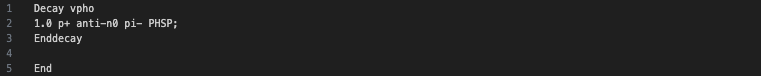
\includegraphics[width=1\textwidth]{appendix/images/dec_file}
    \caption{Decay file example with EvtGen generator.}
    \label{fig:evt_gen_dec}
\end{figure}

The declaration of a decay begins with the keyword \emph{Decay} and ends with \emph{Enddecay}. In this case, the dummy particle \emph{vpho} is costrained to decay into a proton (p+), an antineutron (anti-n0) and a negative pion (pi-) according to the Phase Space Model (PHSP), with branching ratio set to 1.0. Since the channel is the following one:

\begin{center}
$e^+ \ + \  e^- \rightarrow p \ + \ \pi^- \ + \ \bar{n} \  (+ \ \gamma_{ISR})$
\end{center}
In order to produce this specific channel with ISR emission, both \emph{PHOKHARA} and \emph{EvtGen} generators are employed. The first one is acting as ISR generator by generating:

\begin{center}
$e^+ \ + \  e^- \rightarrow vpho \  (+ \ \gamma_{ISR})$
\end{center}

Finally, the virtual photon is decayed by Evt\_Gen, according to the shown above decay file:
\begin{center}
$vpho \rightarrow p \ + \ \pi^- \ + \ \bar{n}$
\end{center}
$\\$
The generation steering file is the operative script that generates a MC sample. An example is given in Fig.~\ref{fig:evt_gen_phokhara}: 

\begin{figure}[H]
    \centering
    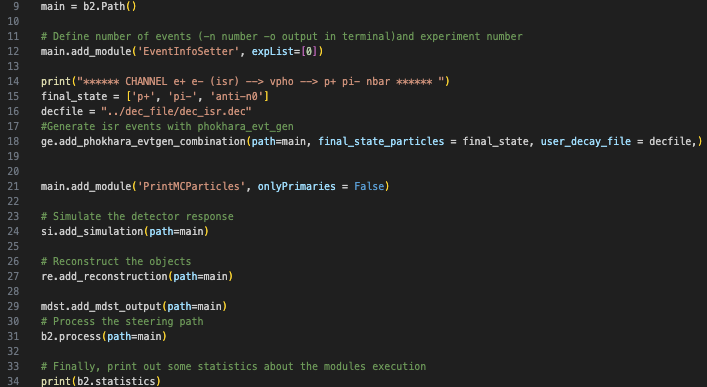
\includegraphics[width=1\textwidth]{appendix/images/gen_file}
    \caption{Usage of PHOKHARA\&Evt\_Gen, where simulation and reconstruction are performed.}
      \label{fig:evt_gen_phokhara}
\end{figure}

The basf2 scripts are structured as modules, which are sequentially arranged within a path, which is called \emph{main} in this example (row9). The first module (row 12) sets the desired amount of events and the specific experiment number, which is provided via keyboard input prior to script interpretation. Then, the signal from the decay file is added (row 18), with add\_phokhara\_evtgen\_combination from generators basf2 modules \footnote{https://software.belle2.org/development/sphinx/generators/doc/index.html}. From row 24 to 27, the simulation and the reconstruction, are added to the path. Then the output file is created to store the MC truth, namely the generated event with a specific signal sample. Finally the steering path is processed in row 31. 
\clearpage
Cluster variables in ISR case:
 \begin{figure}[H]
    \centering
    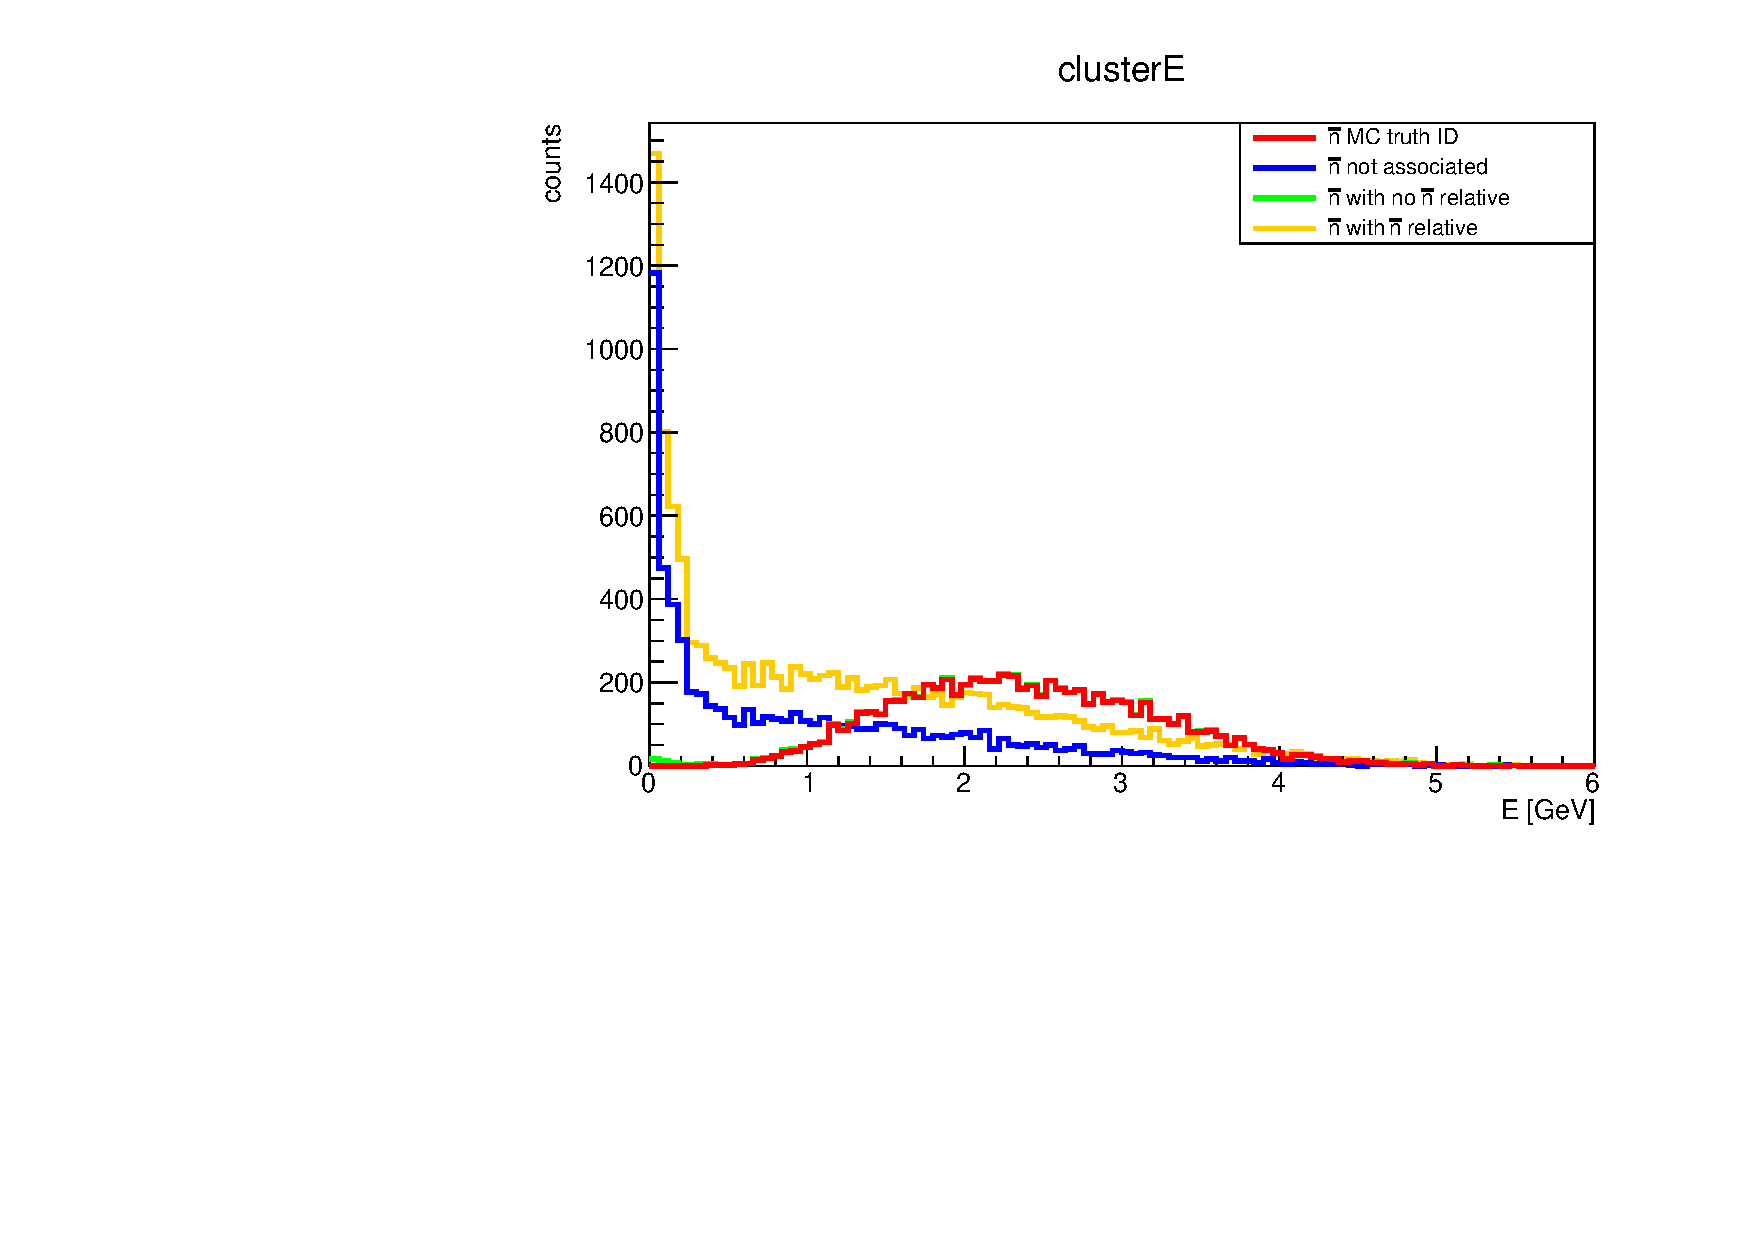
\includegraphics[width=0.49\textwidth]{nbar_MC/images/clusterE_isr_ancestor.pdf}
    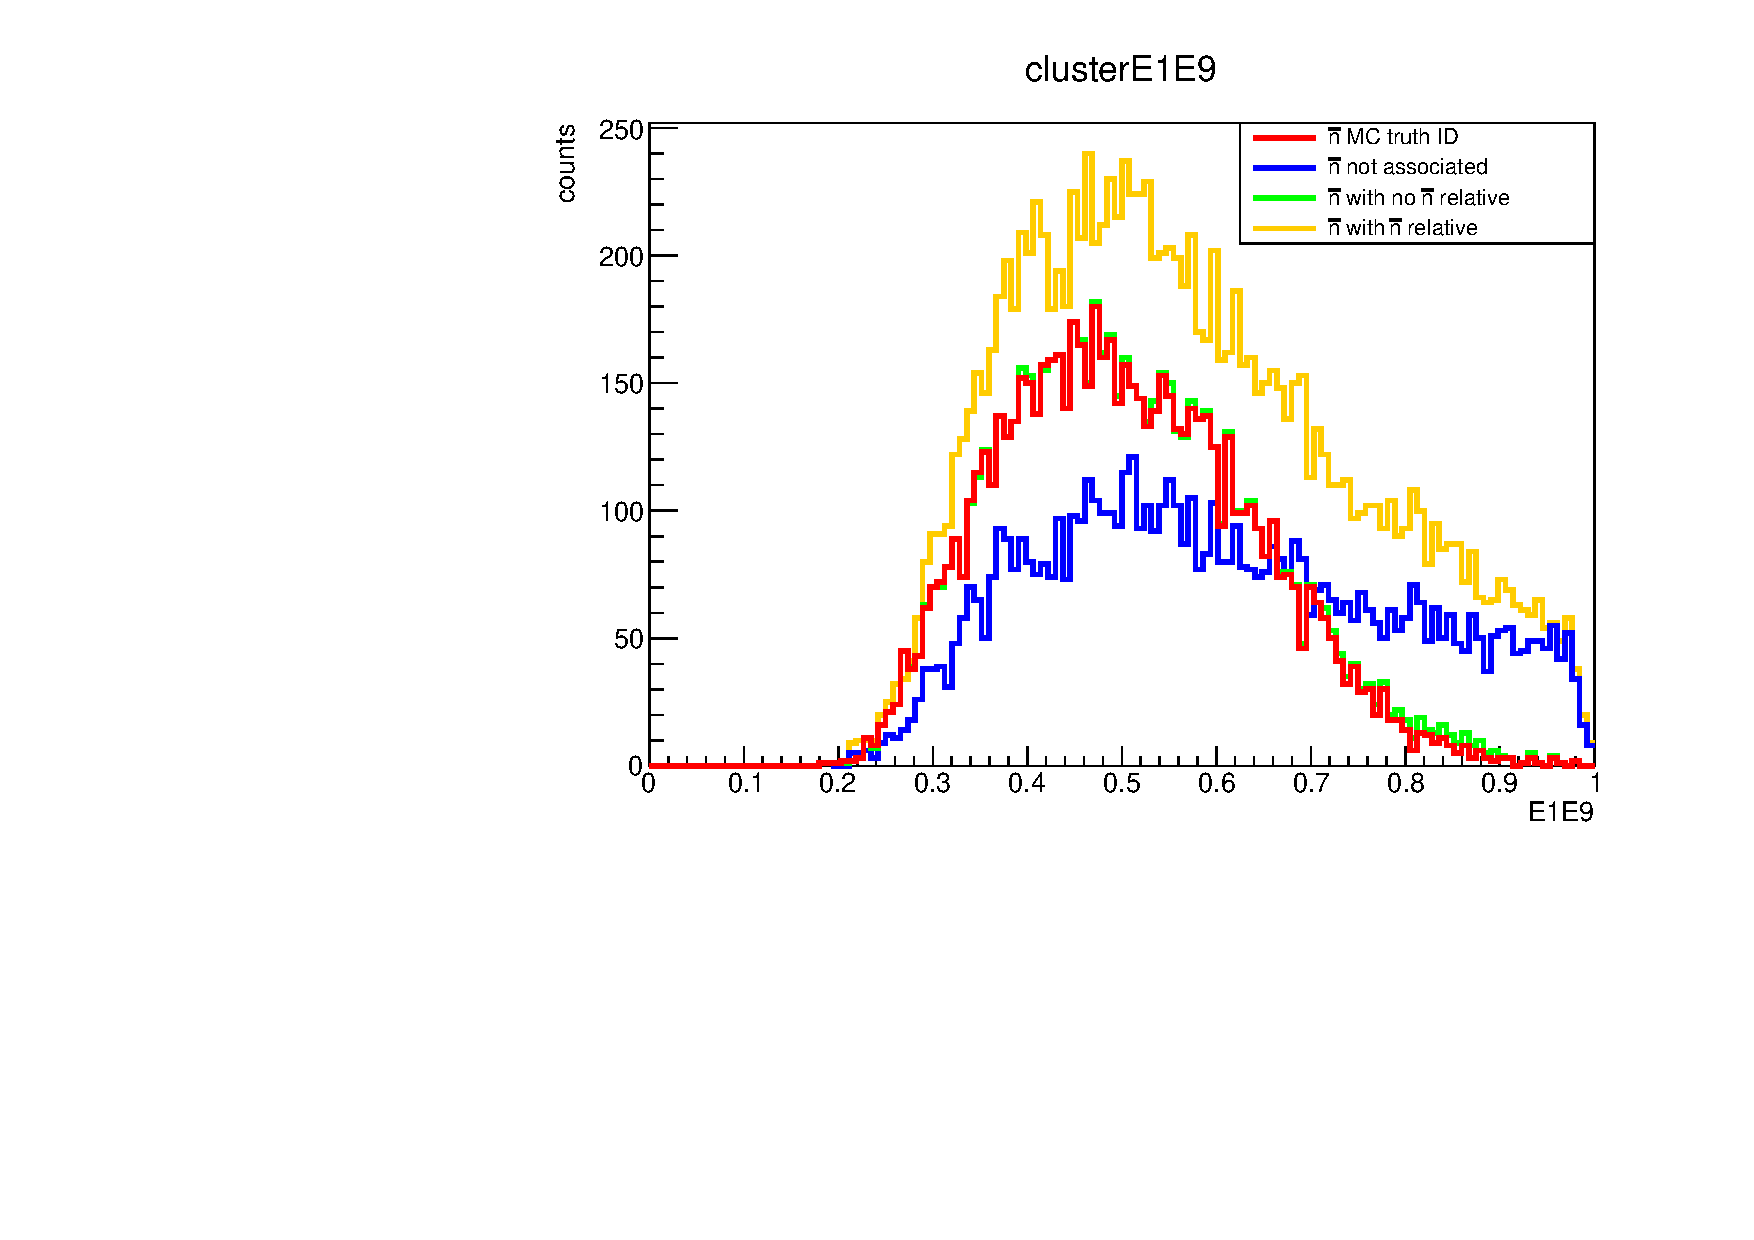
\includegraphics[width=0.49\textwidth]{nbar_MC/images/clusterE1E9_isr_ancestor.pdf}
    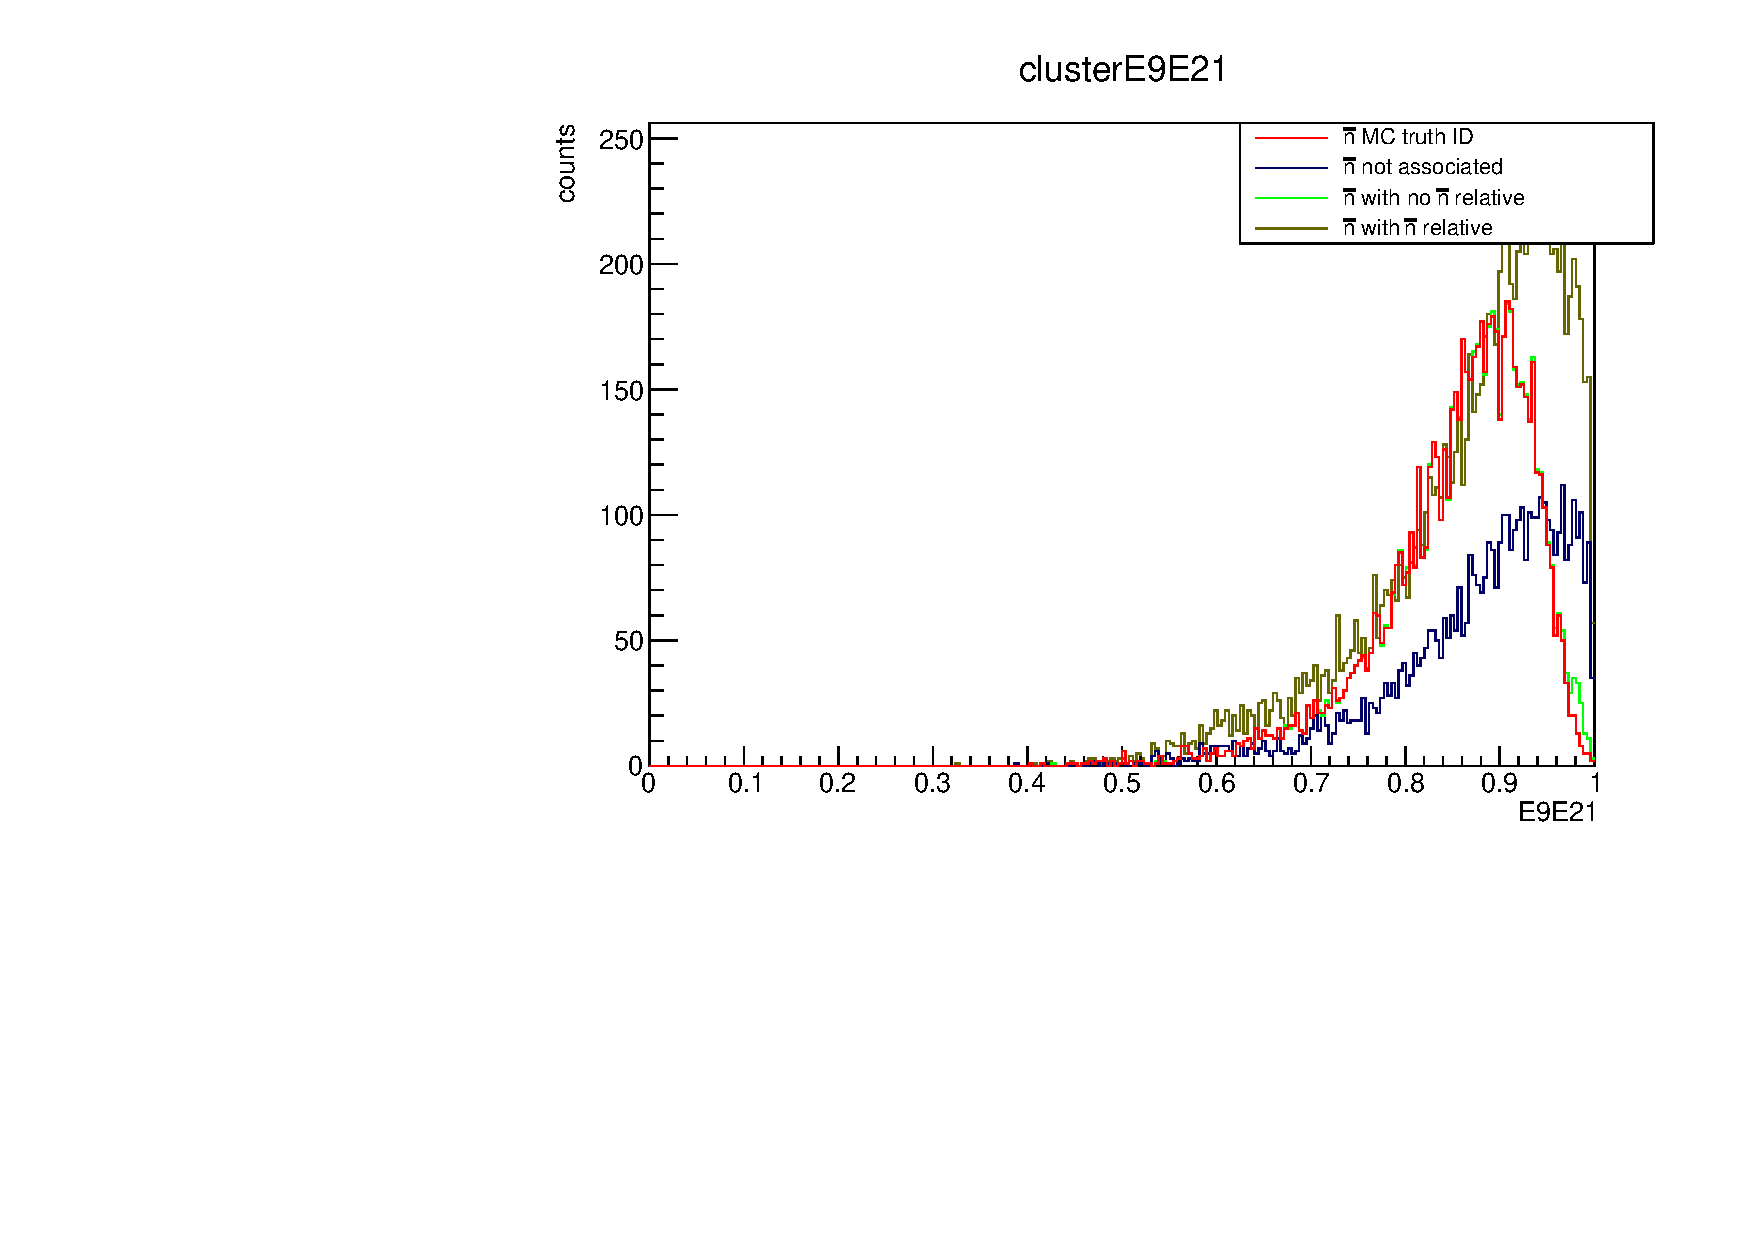
\includegraphics[width=0.49\textwidth]{nbar_MC/images/clusterE9E21_isr_ancestor.pdf}
    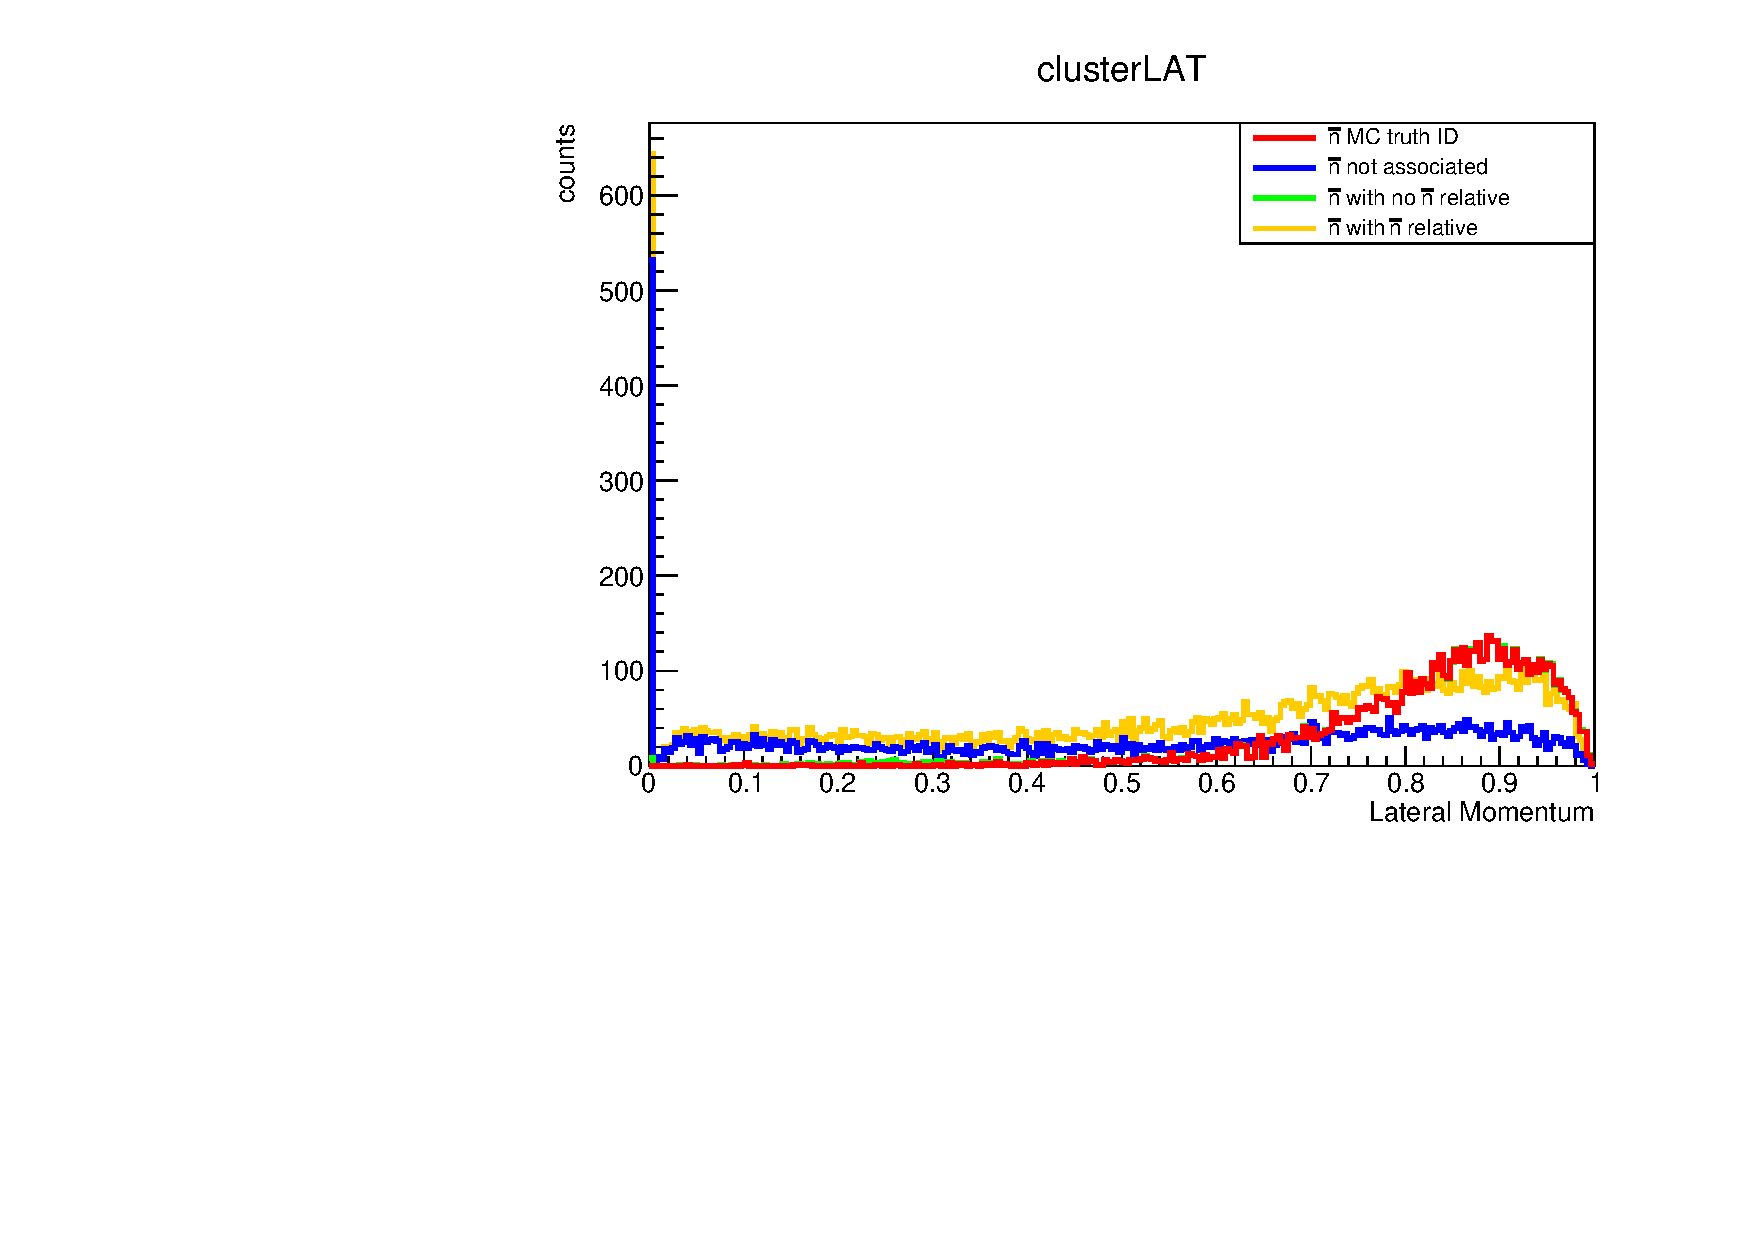
\includegraphics[width=0.49\textwidth]{nbar_MC/images/clusterLAT_isr_ancestor.pdf}
    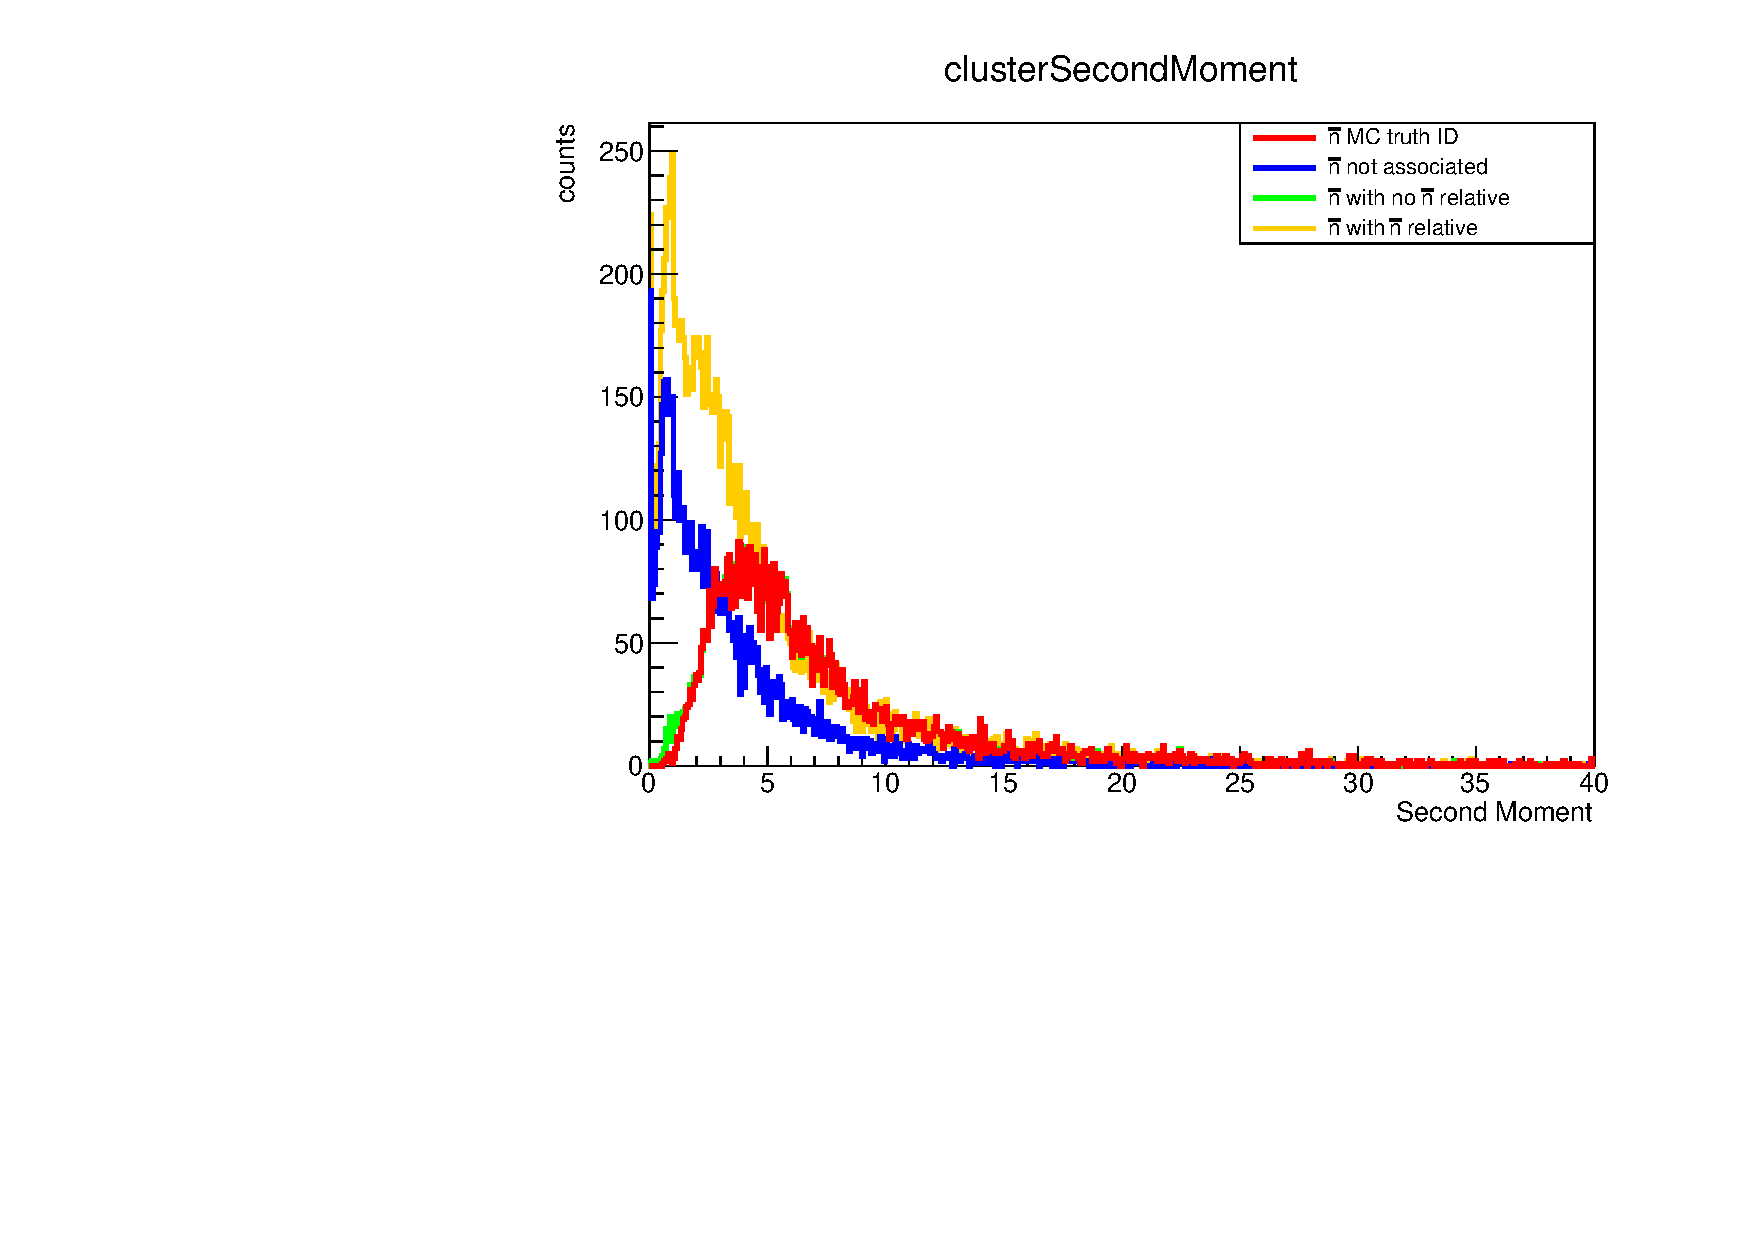
\includegraphics[width=0.49\textwidth]{nbar_MC/images/clusterSecondMoment_isr_ancestor.pdf}
    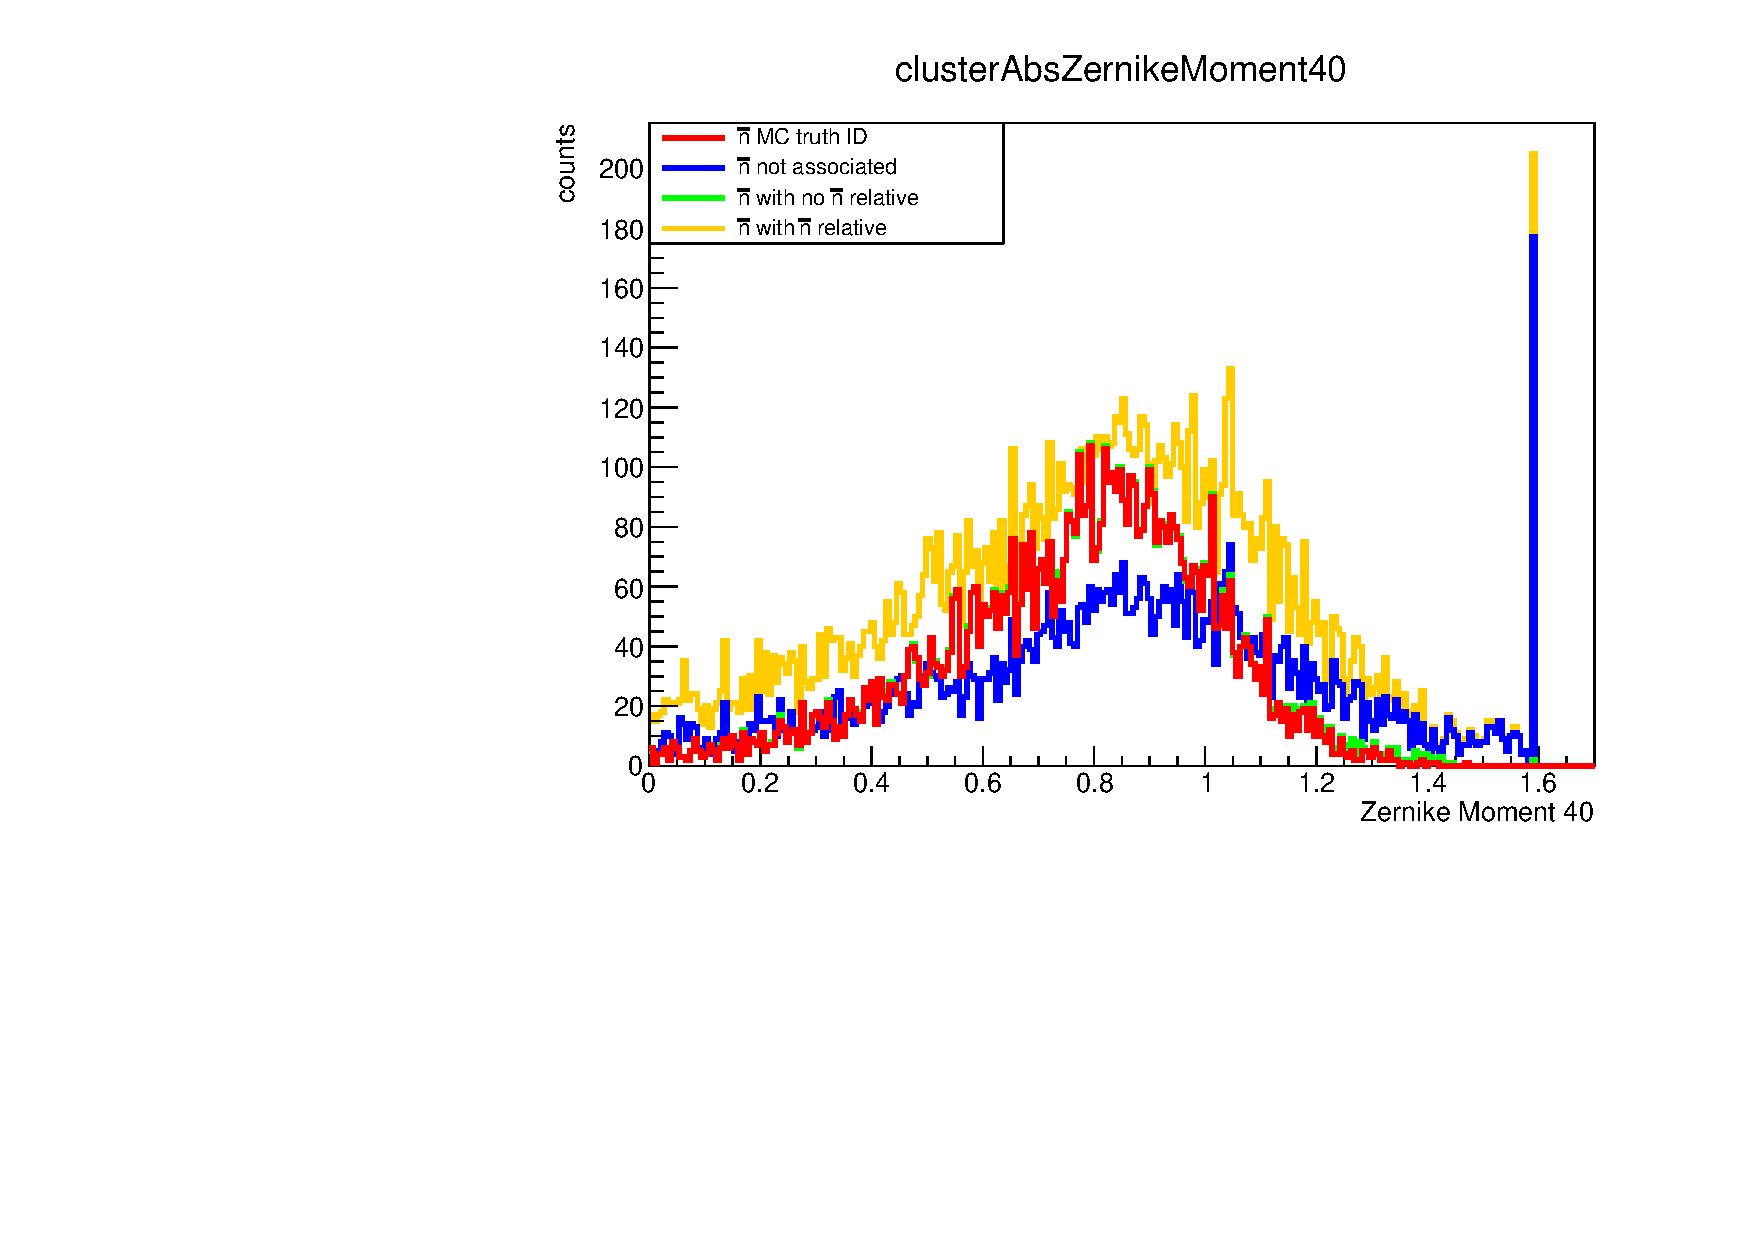
\includegraphics[width=0.49\textwidth]{nbar_MC/images/clusterAbsZernikeMoment40_isr_ancestor.pdf}
    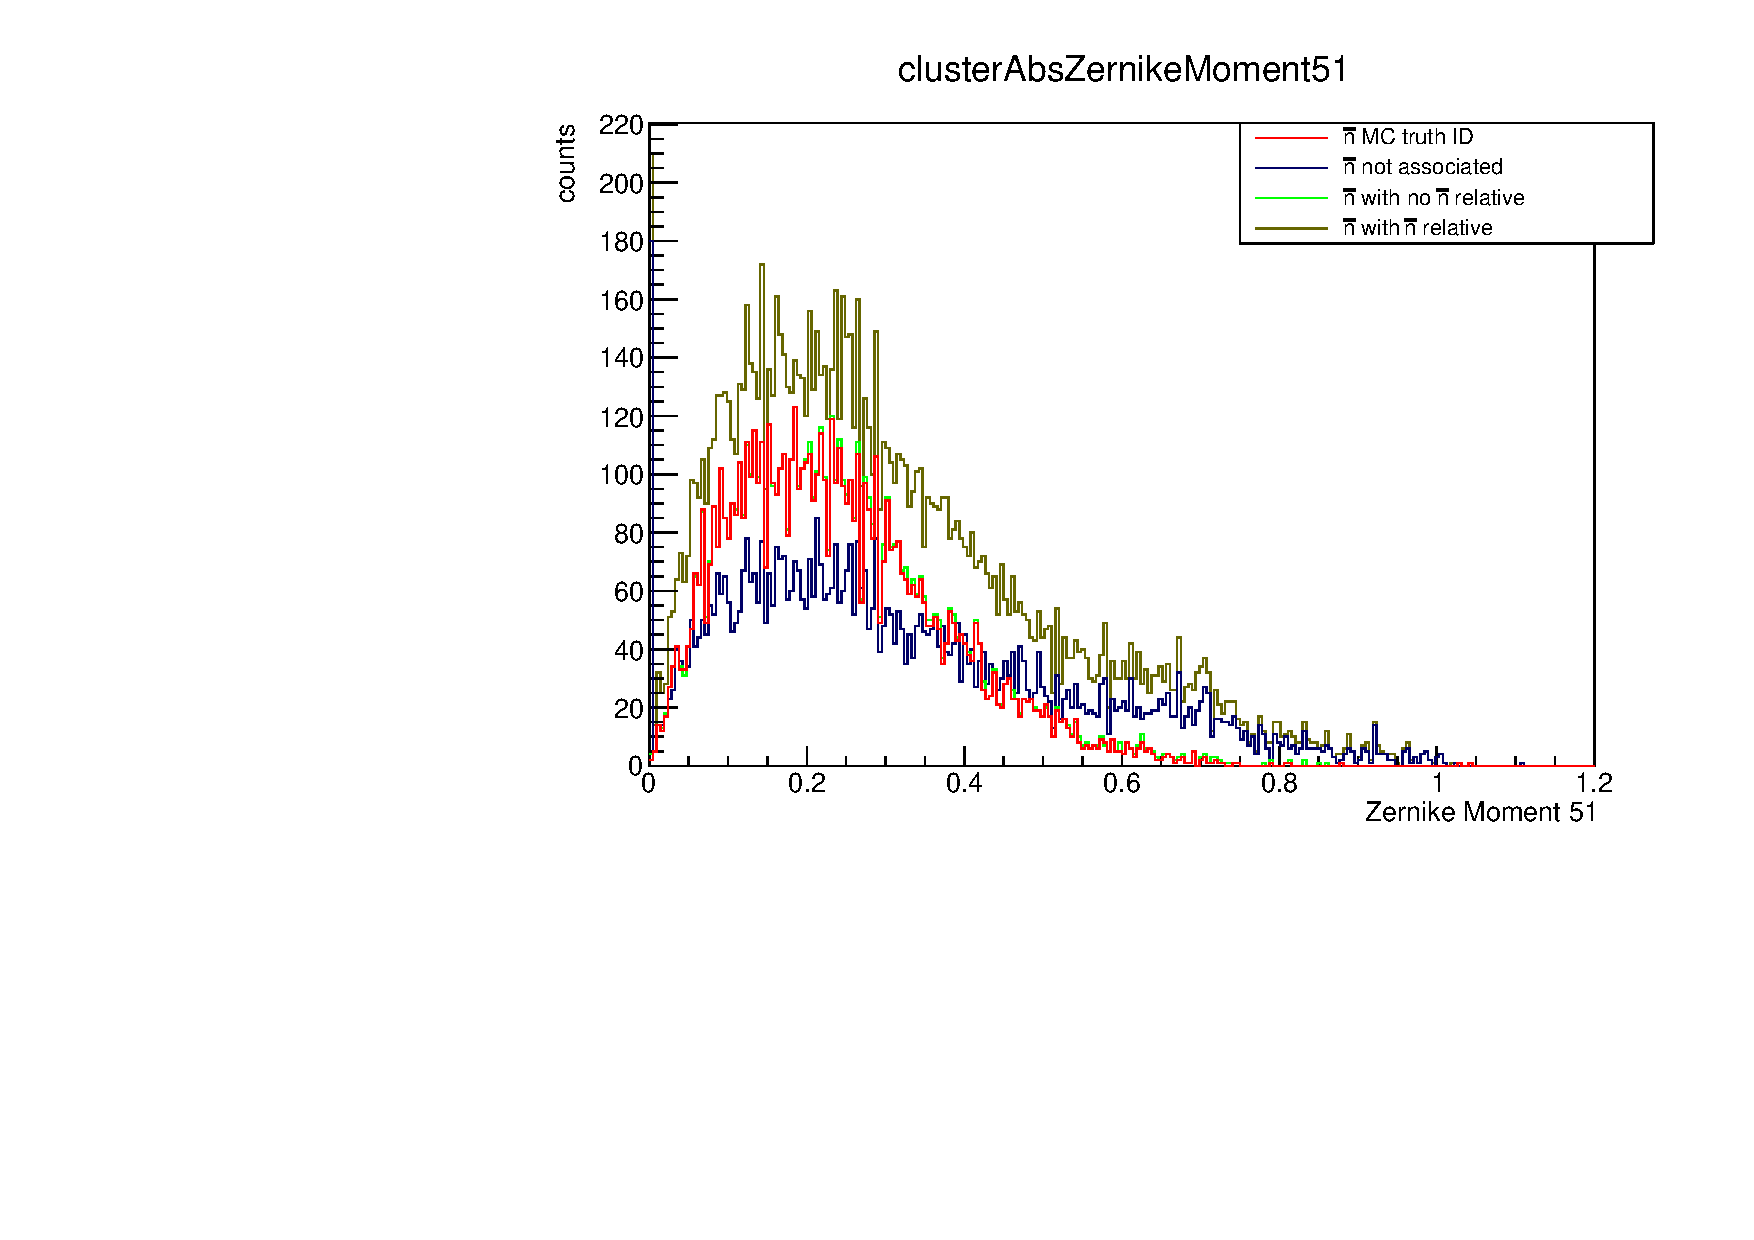
\includegraphics[width=0.49\textwidth]{nbar_MC/images/clusterAbsZernikeMoment51_isr_ancestor.pdf}
    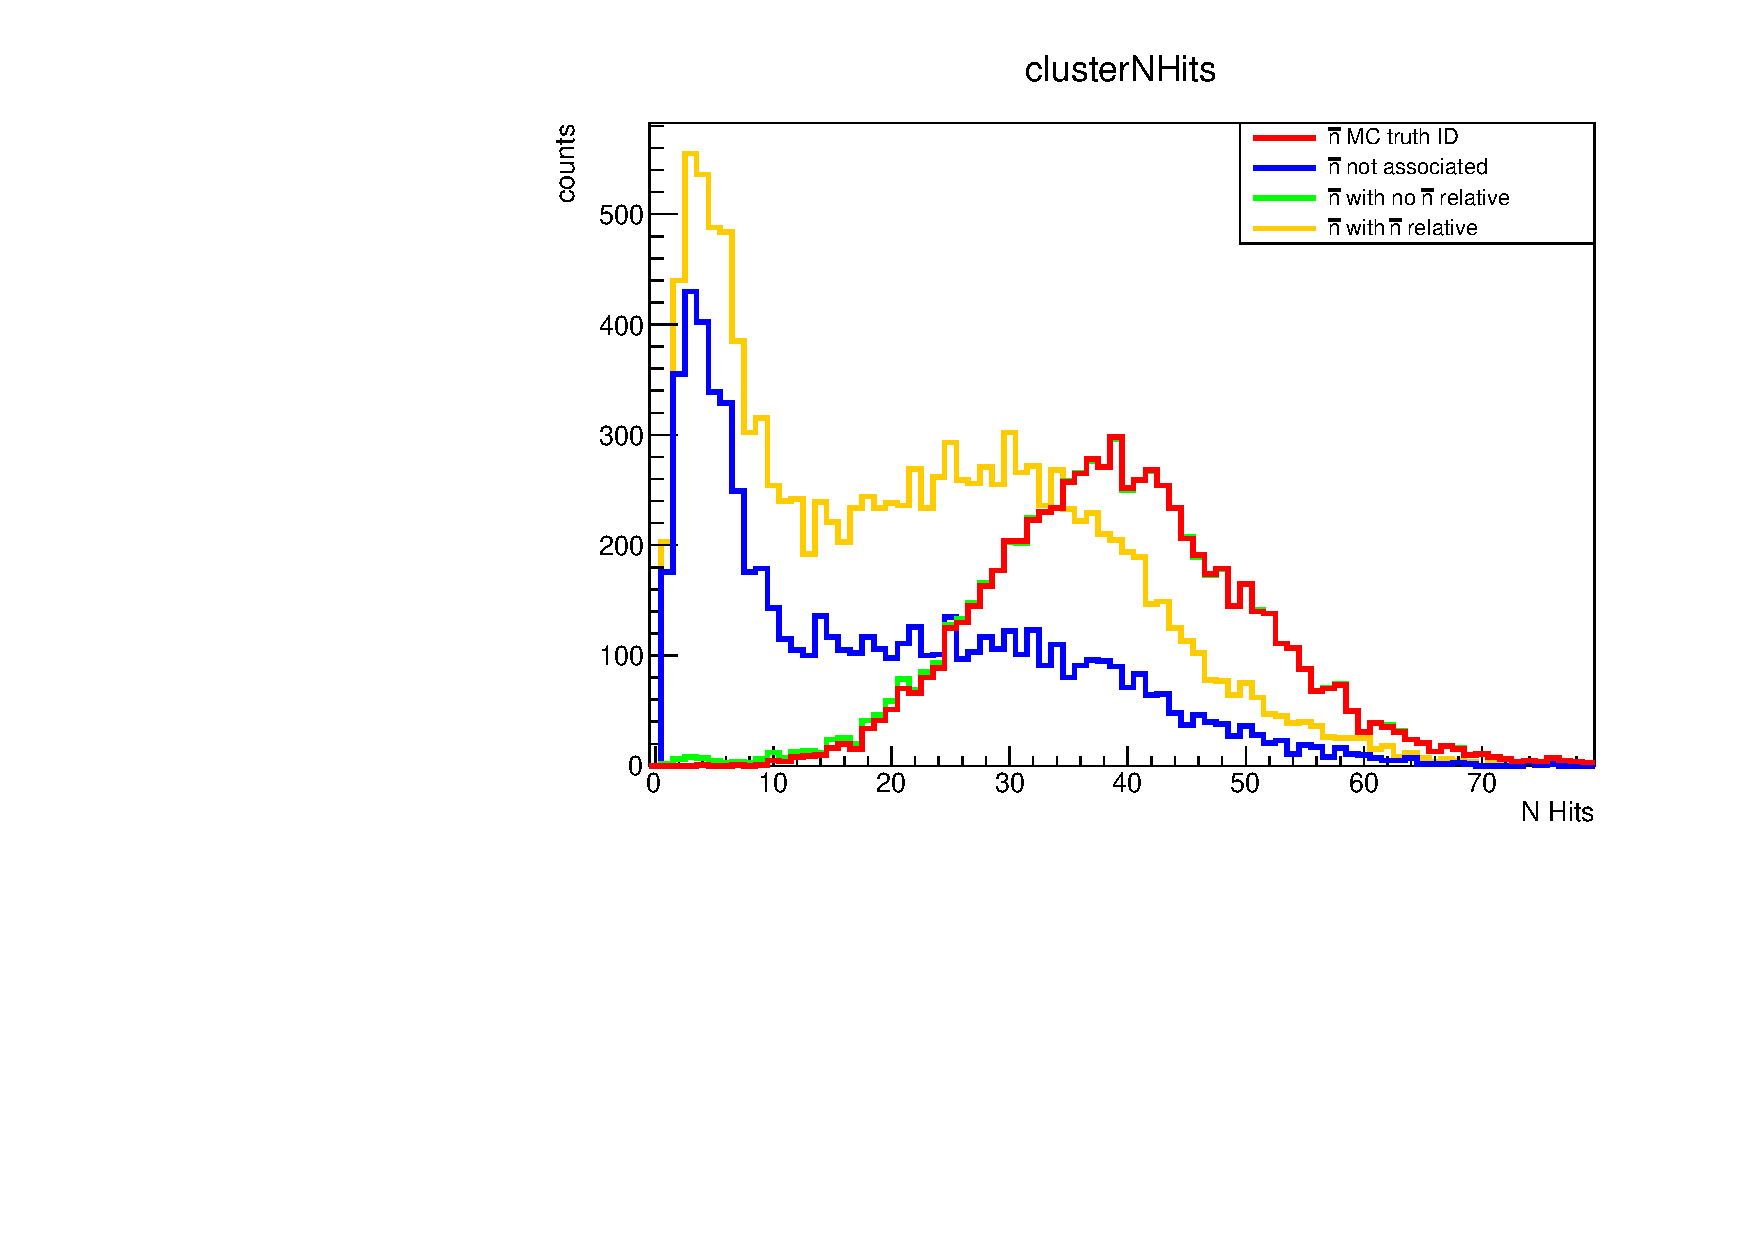
\includegraphics[width=0.49\textwidth]{nbar_MC/images/clusterNHits_isr_ancestor.pdf}
   
   \caption{\footnotesize{Comparison of reconstructed cluster variables for $\bar{n}$ candidates with different ancestor selection (ISR case). Red: $\bar{n}$ candidates associated with true $\bar{n}$ by Monte Carlo matching; blue: $\bar{n}$ candidates not associated with any particle (NaN); green: $\bar{n}$ candidates without $\bar{n}$ relatives; yellow: $\bar{n}$ candidates with $\bar{n}$ relative. The third contribution (green) is barely visible as it lies beneath the first distribution (red). ISR case.}}
     \label{fig:cluster_ISR}
\end{figure}

 \begin{figure}[H]
    \centering
    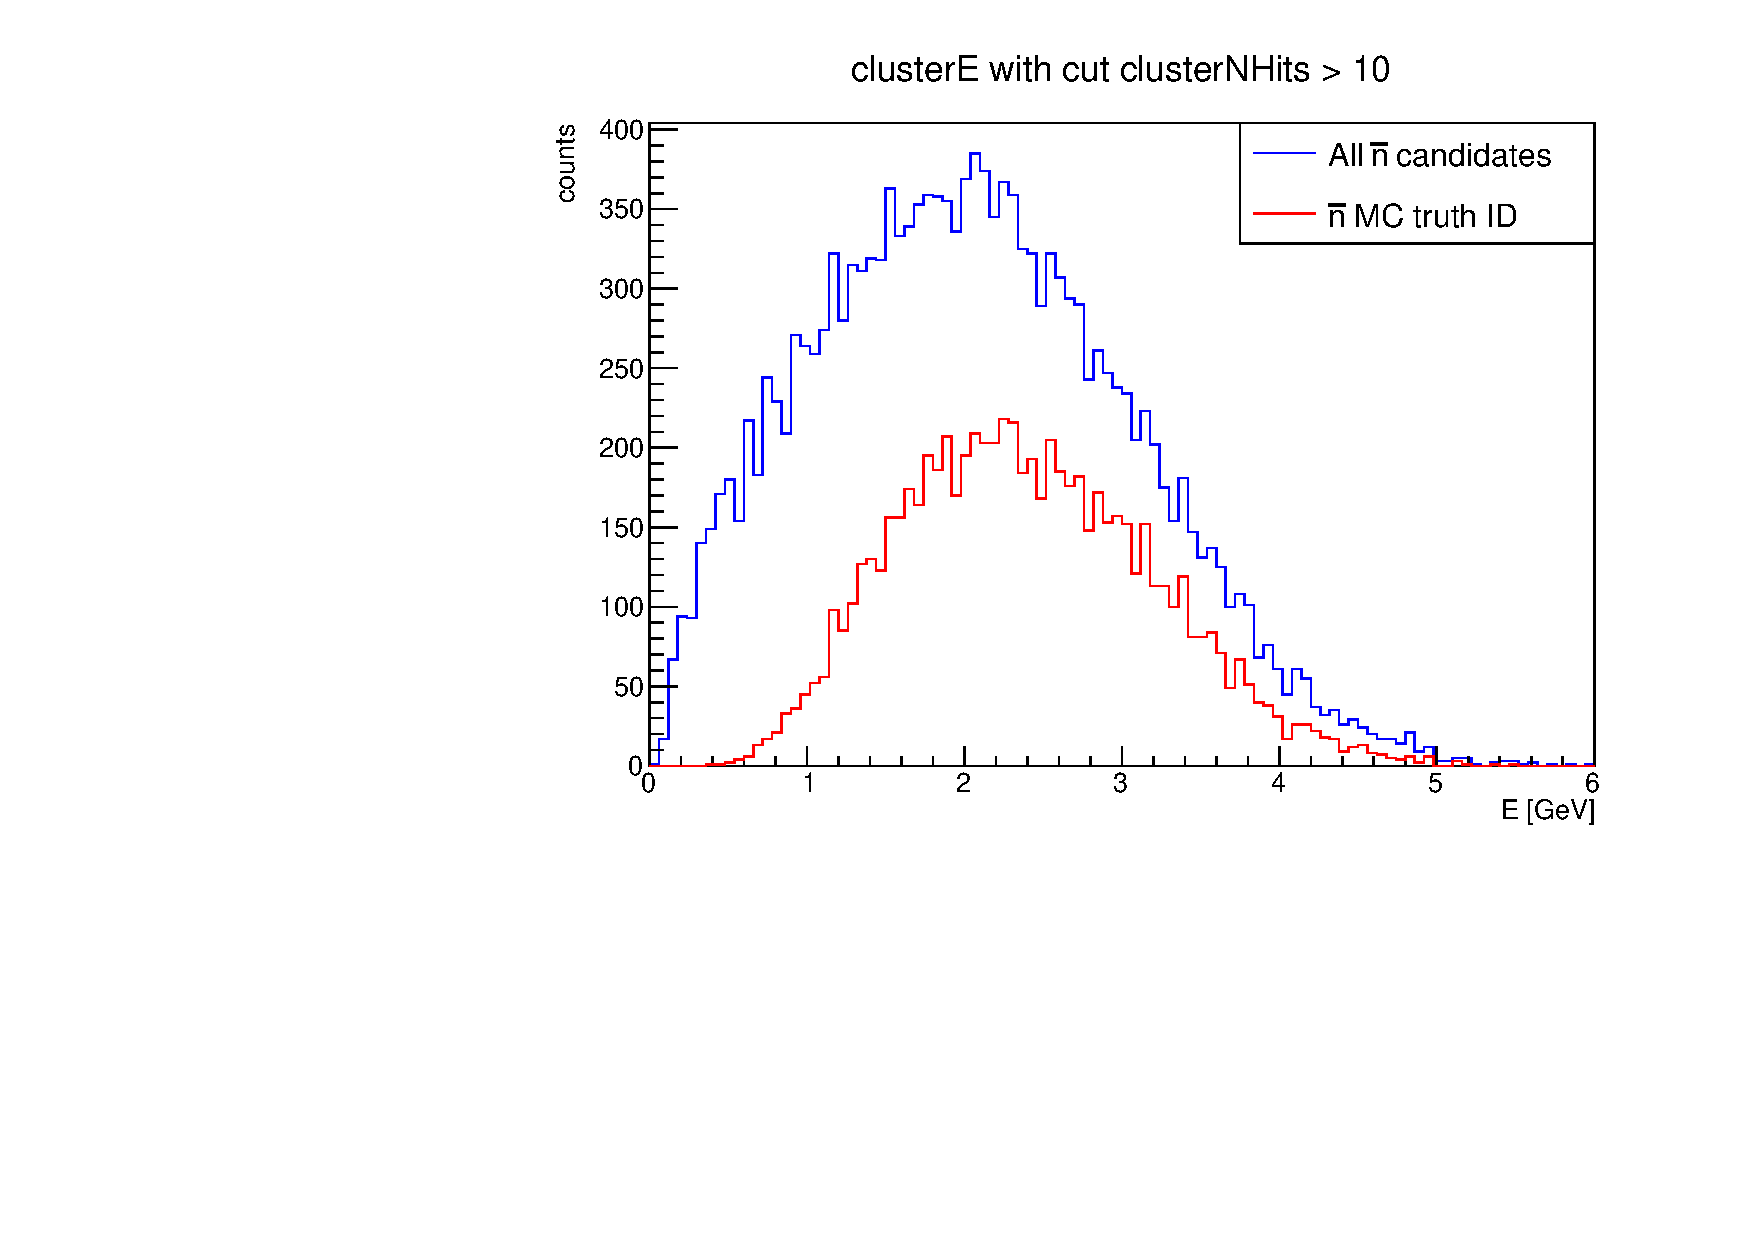
\includegraphics[width=0.49\textwidth]{nbar_MC/images/clusterE_hitscut_isr.pdf}
    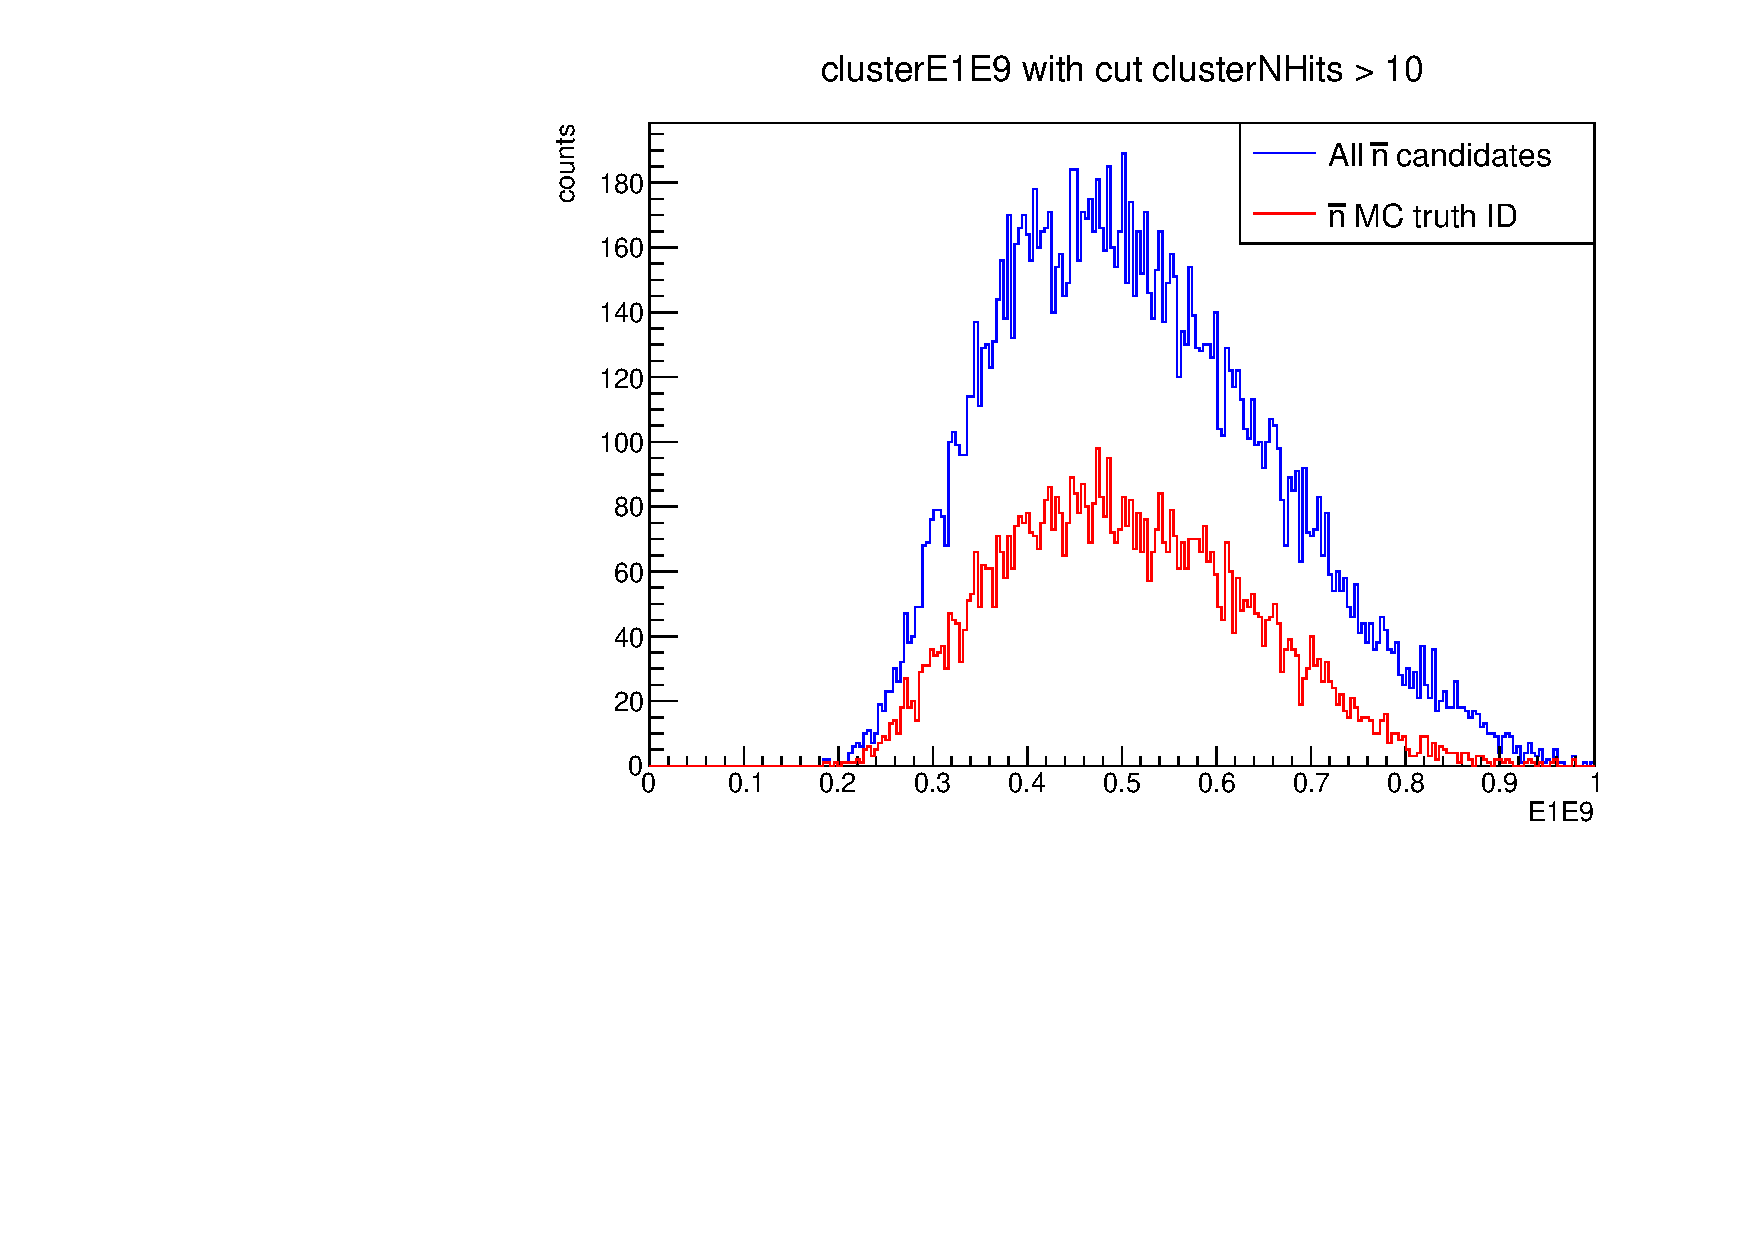
\includegraphics[width=0.49\textwidth]{nbar_MC/images/clusterE1E9_hitscut_isr.pdf}
    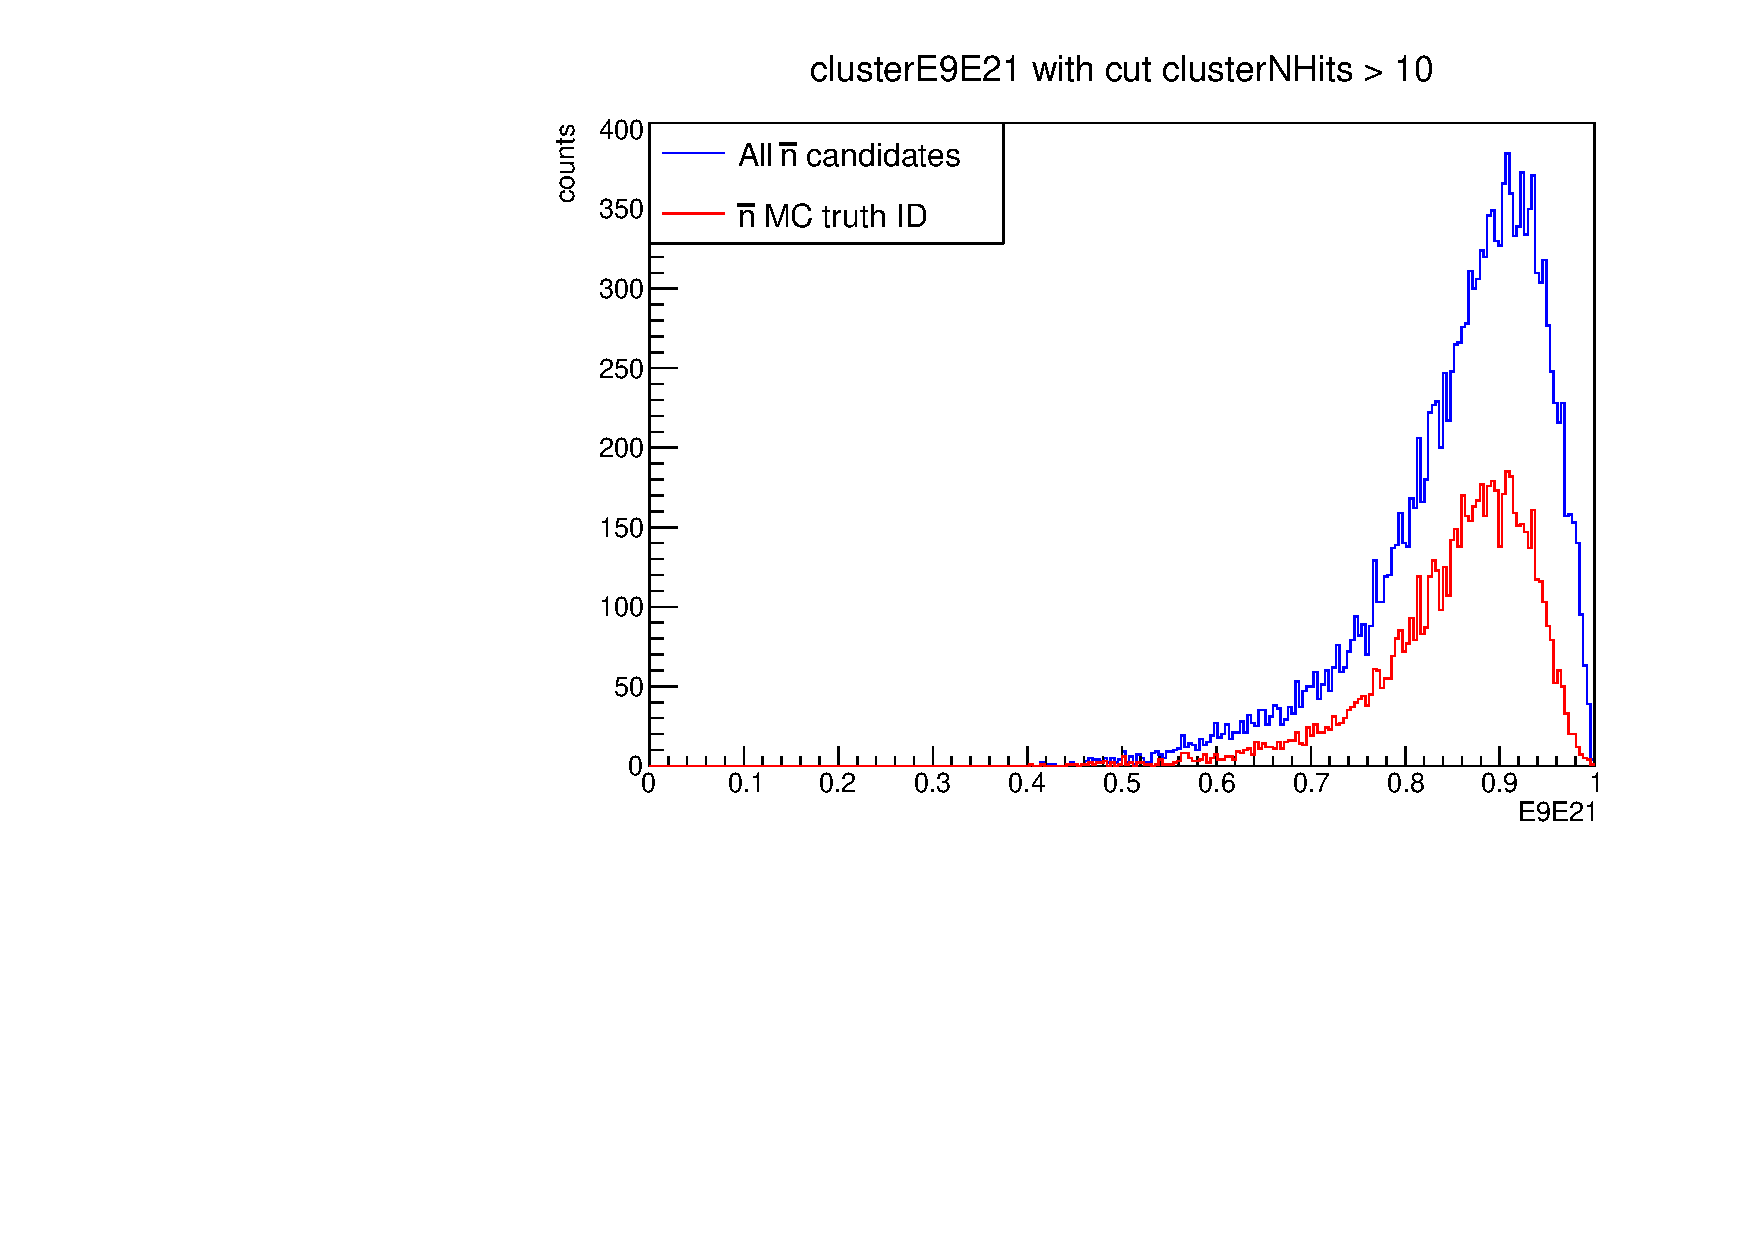
\includegraphics[width=0.49\textwidth]{nbar_MC/images/clusterE9E21_hitscut_isr.pdf}
    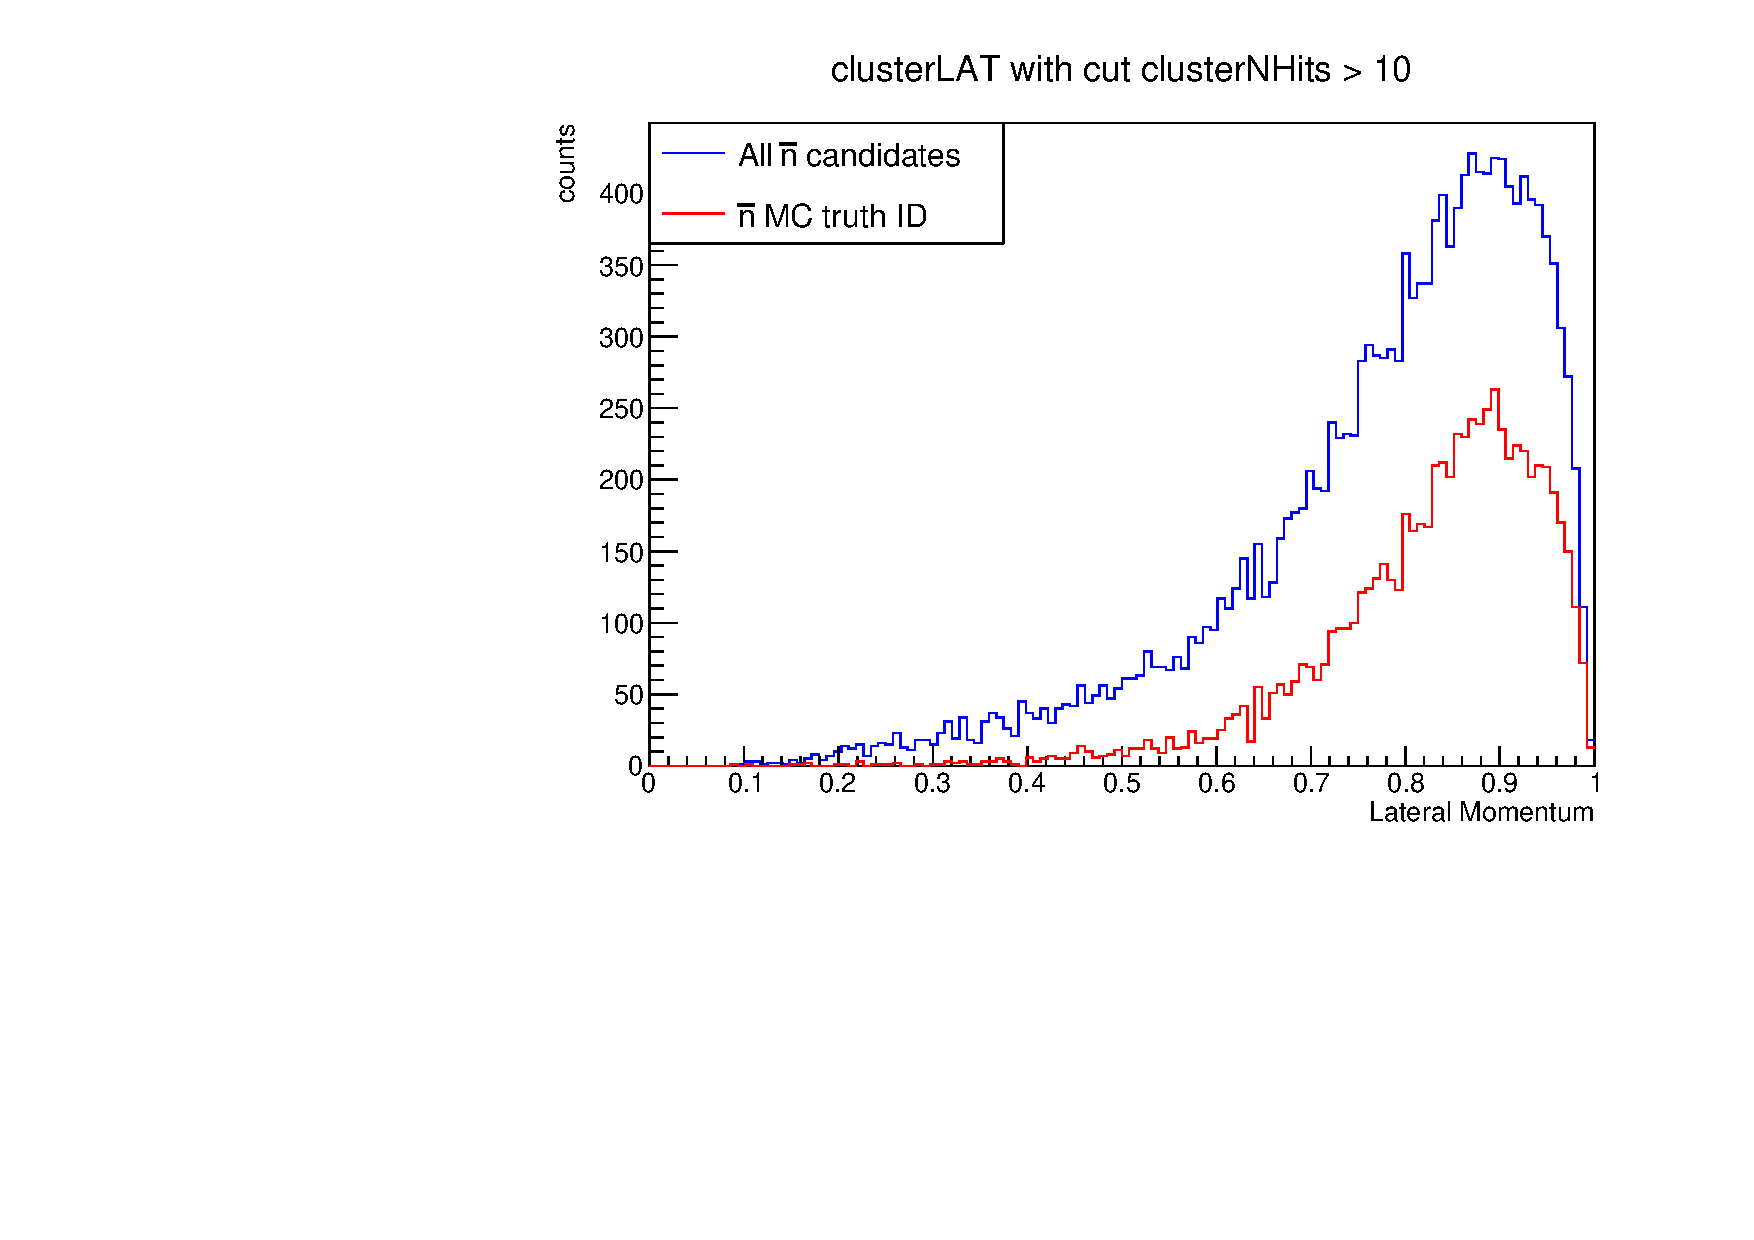
\includegraphics[width=0.49\textwidth]{nbar_MC/images/clusterLAT_hitscut_isr.pdf}
    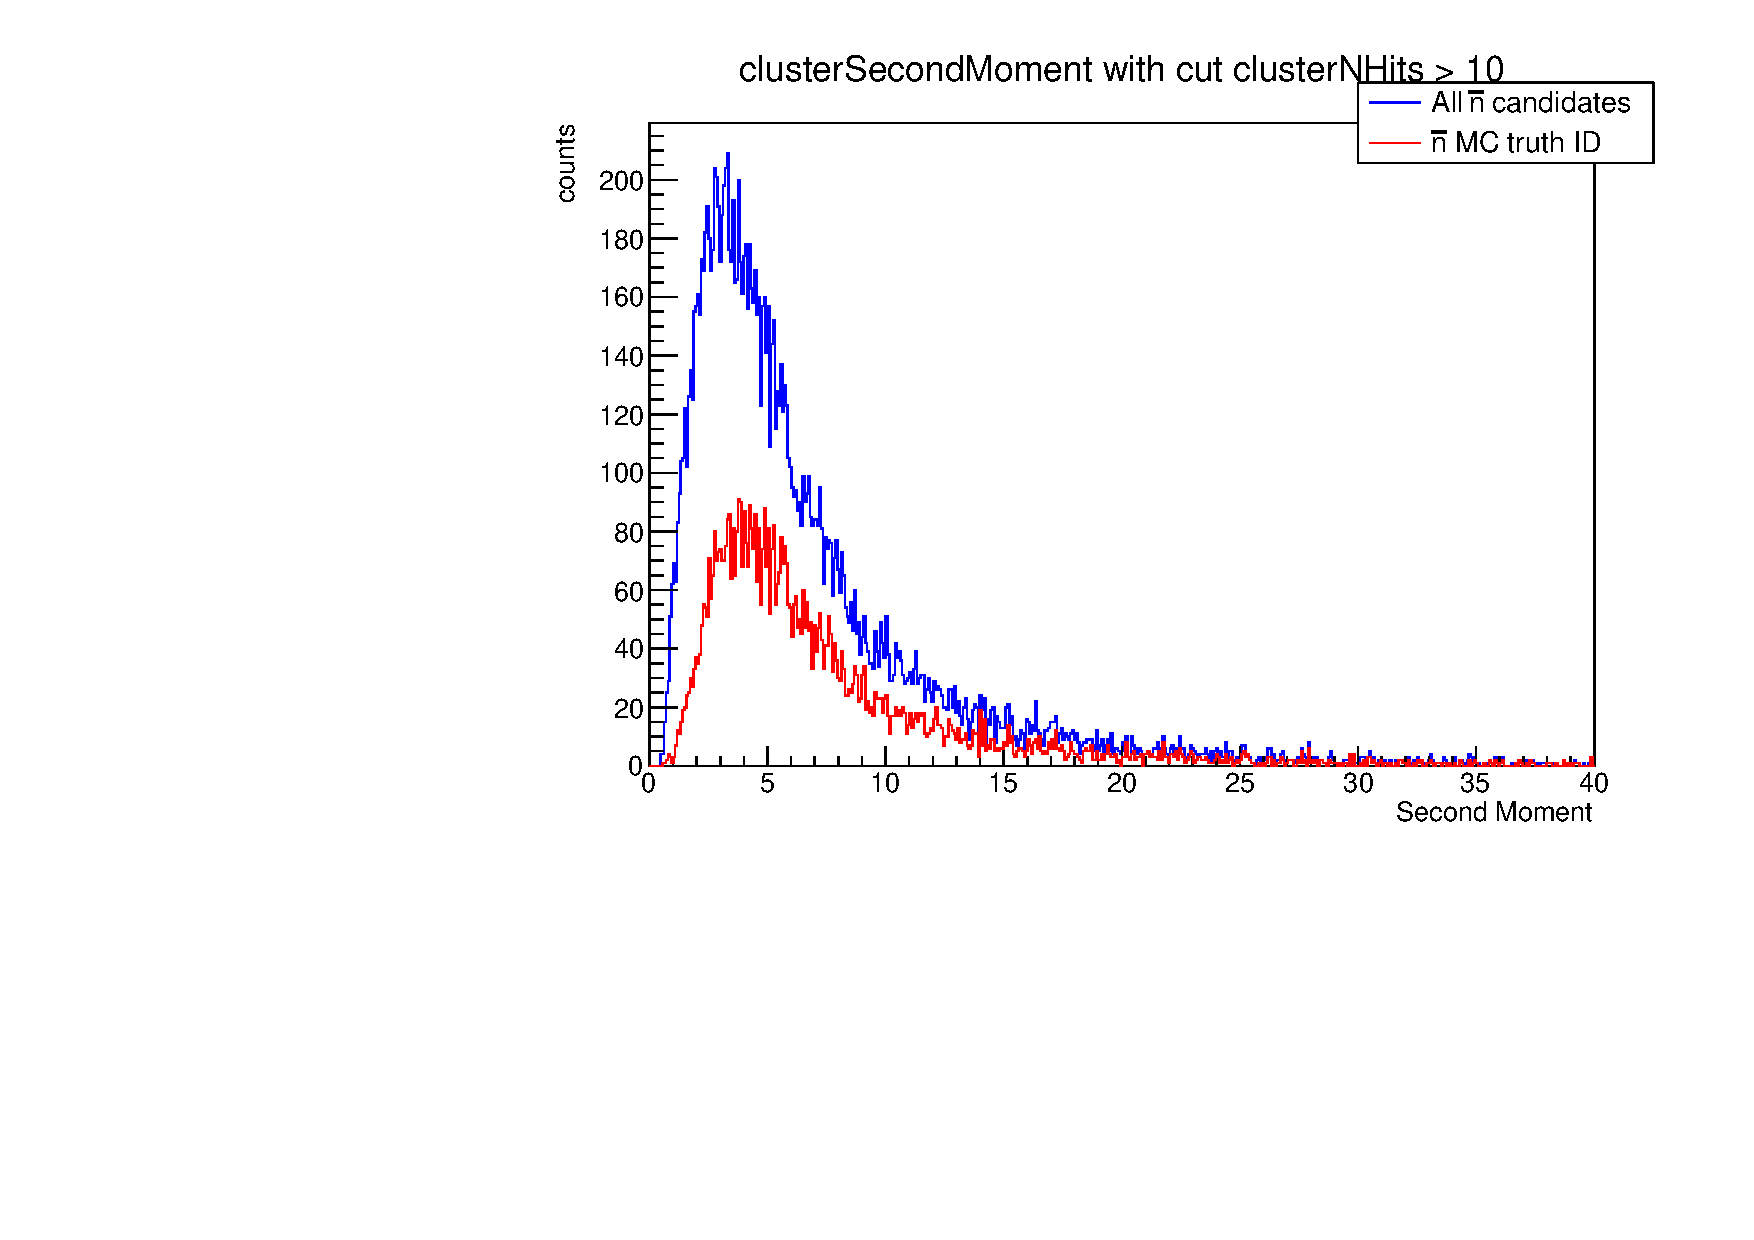
\includegraphics[width=0.49\textwidth]{nbar_MC/images/clusterSecondMoment_hitscut_isr.pdf}
    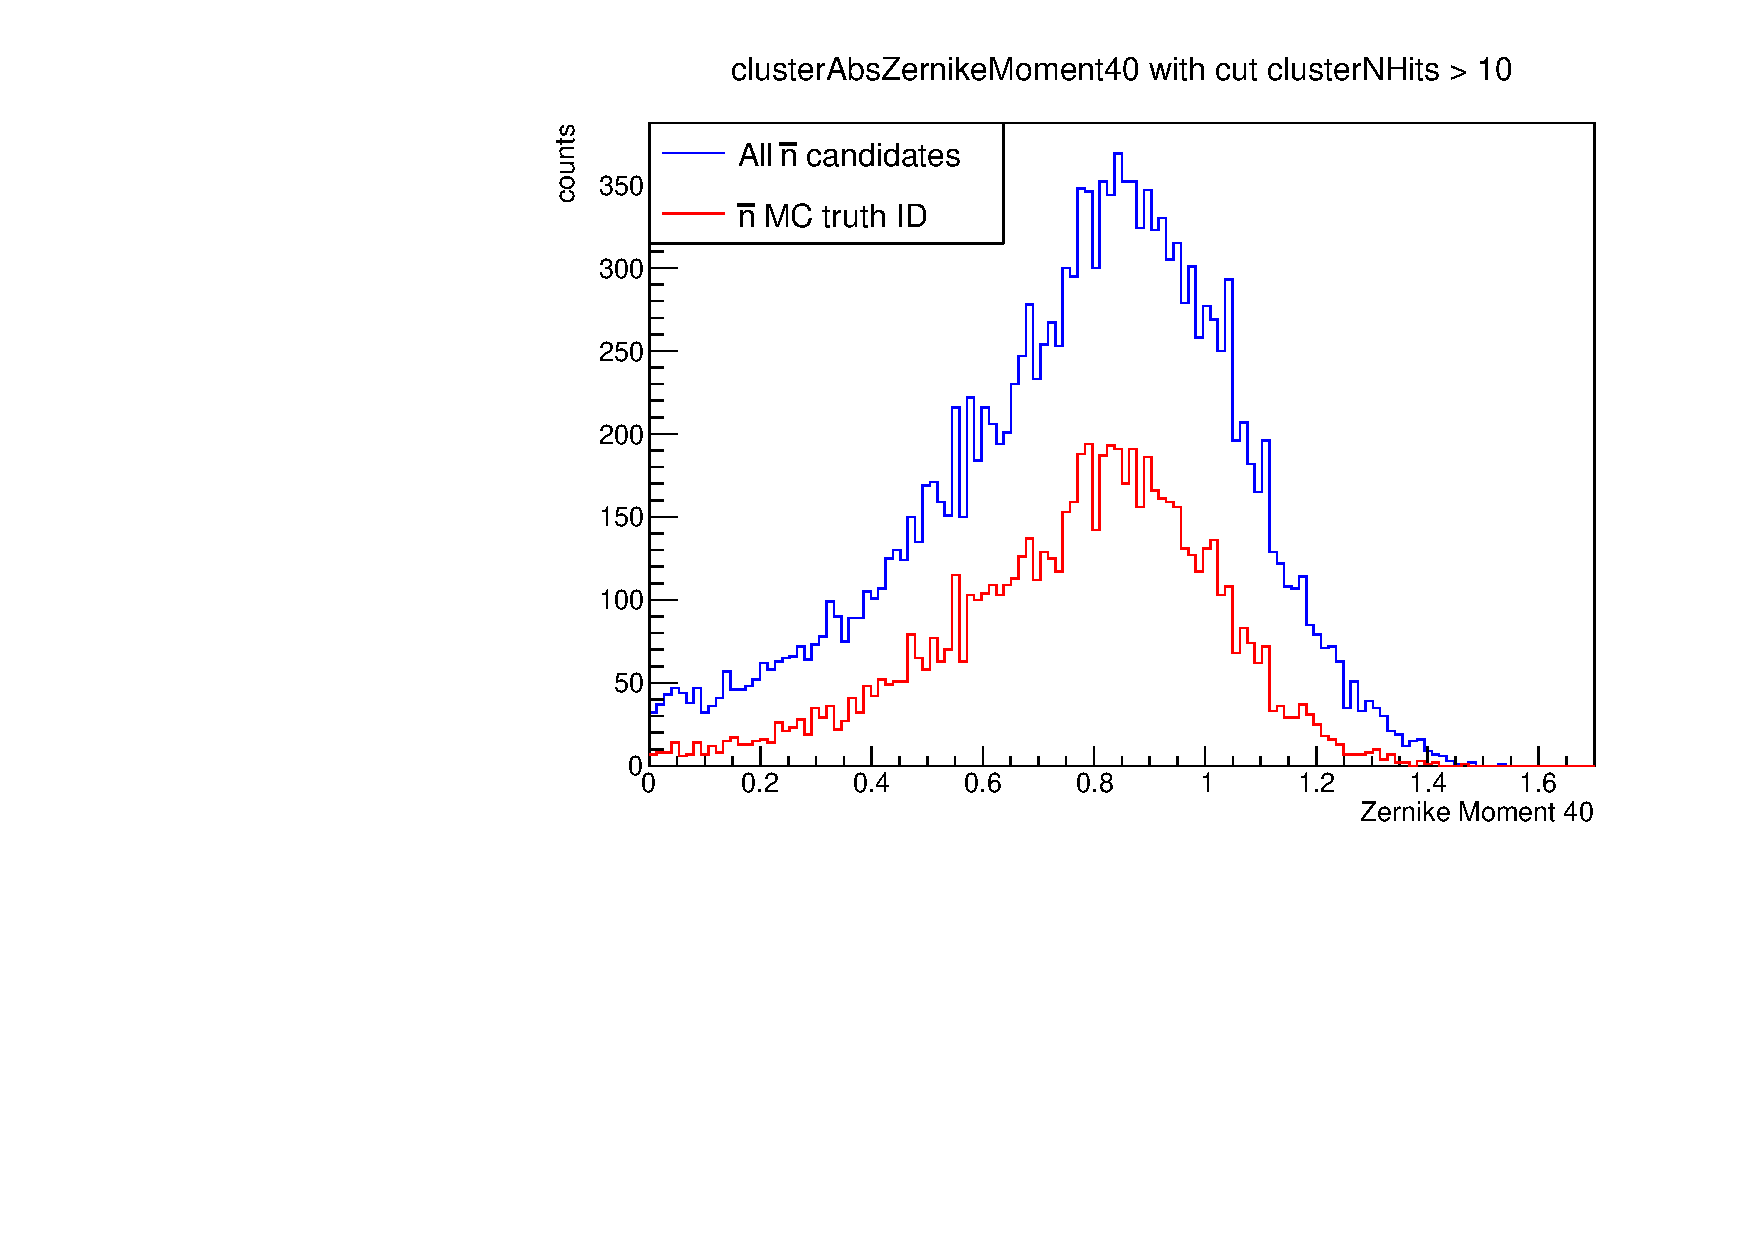
\includegraphics[width=0.49\textwidth]{nbar_MC/images/clusterAbsZernikeMoment40_hitscut_isr.pdf}
    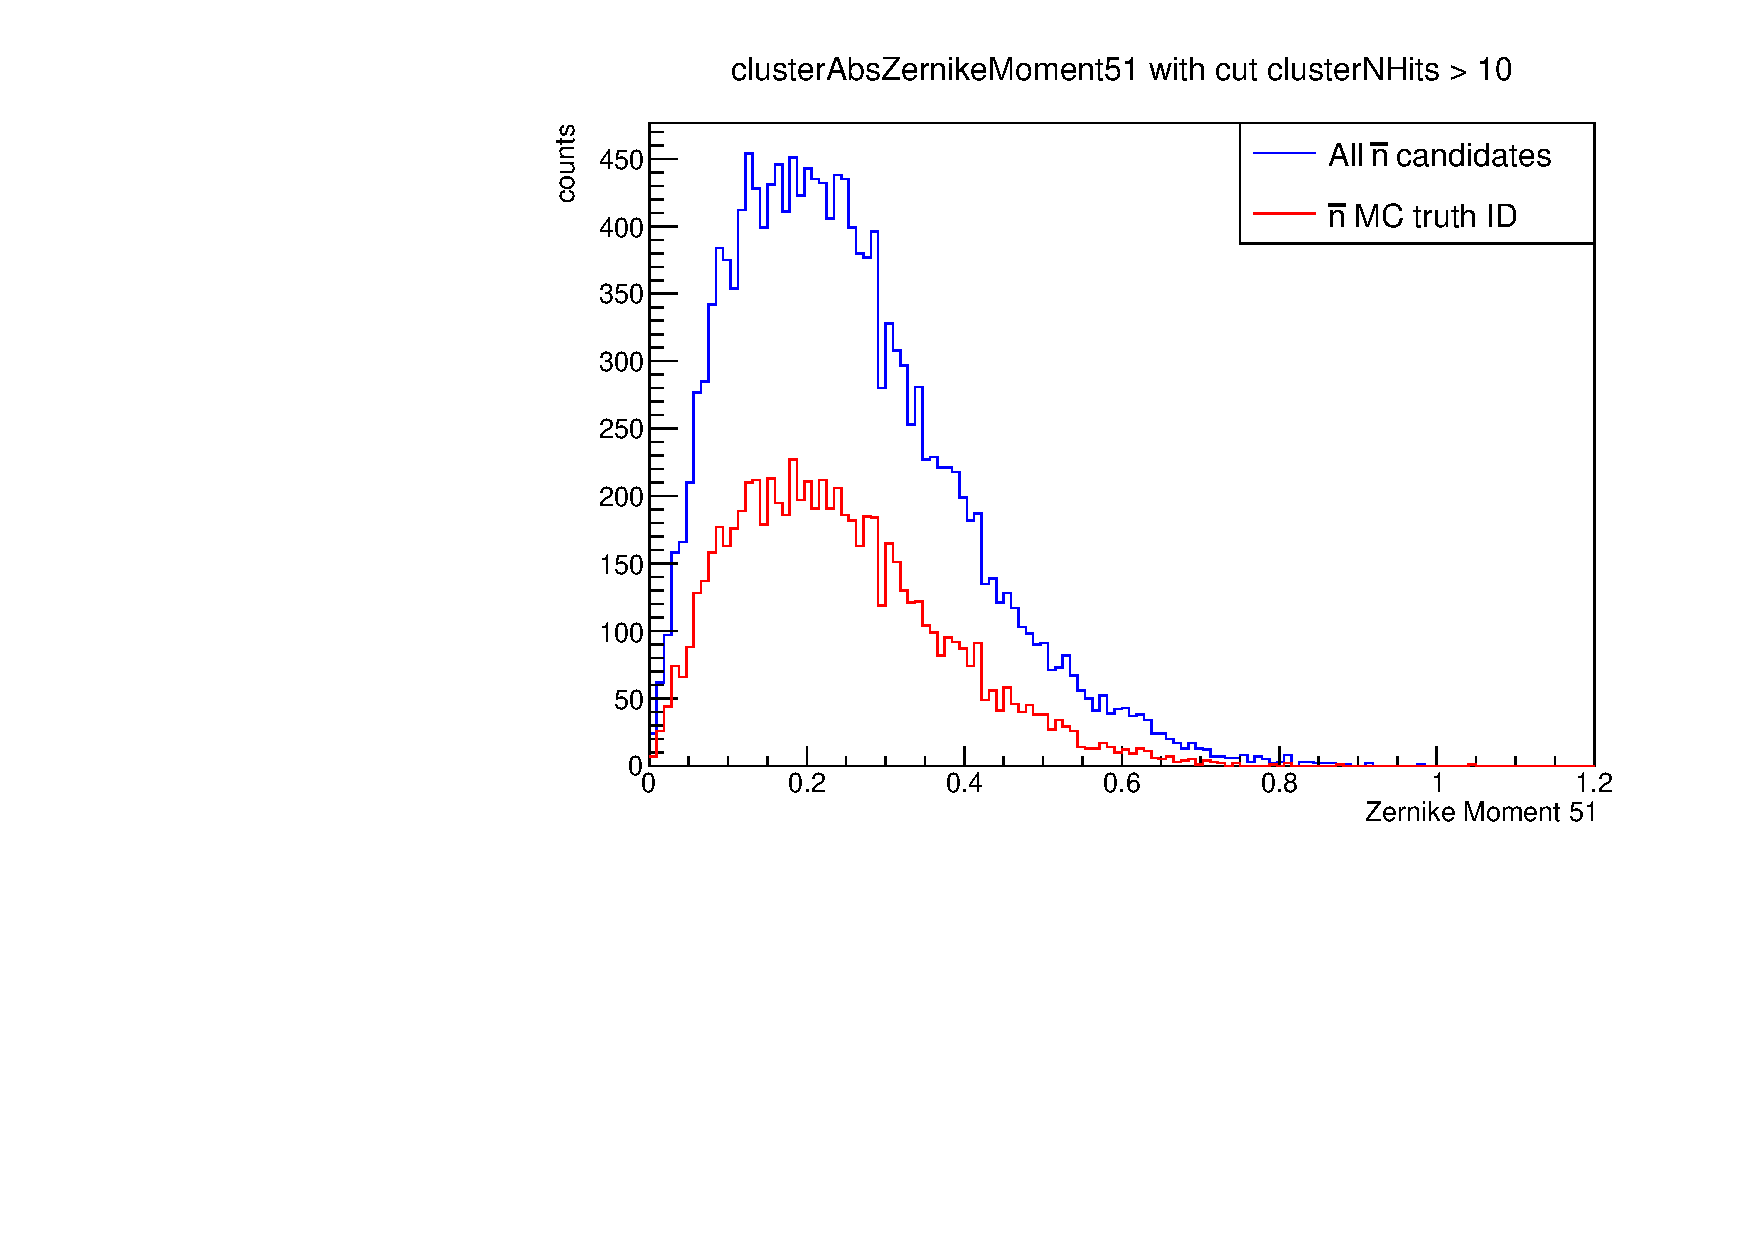
\includegraphics[width=0.49\textwidth]{nbar_MC/images/clusterAbsZernikeMoment51_hitscut_isr.pdf}
    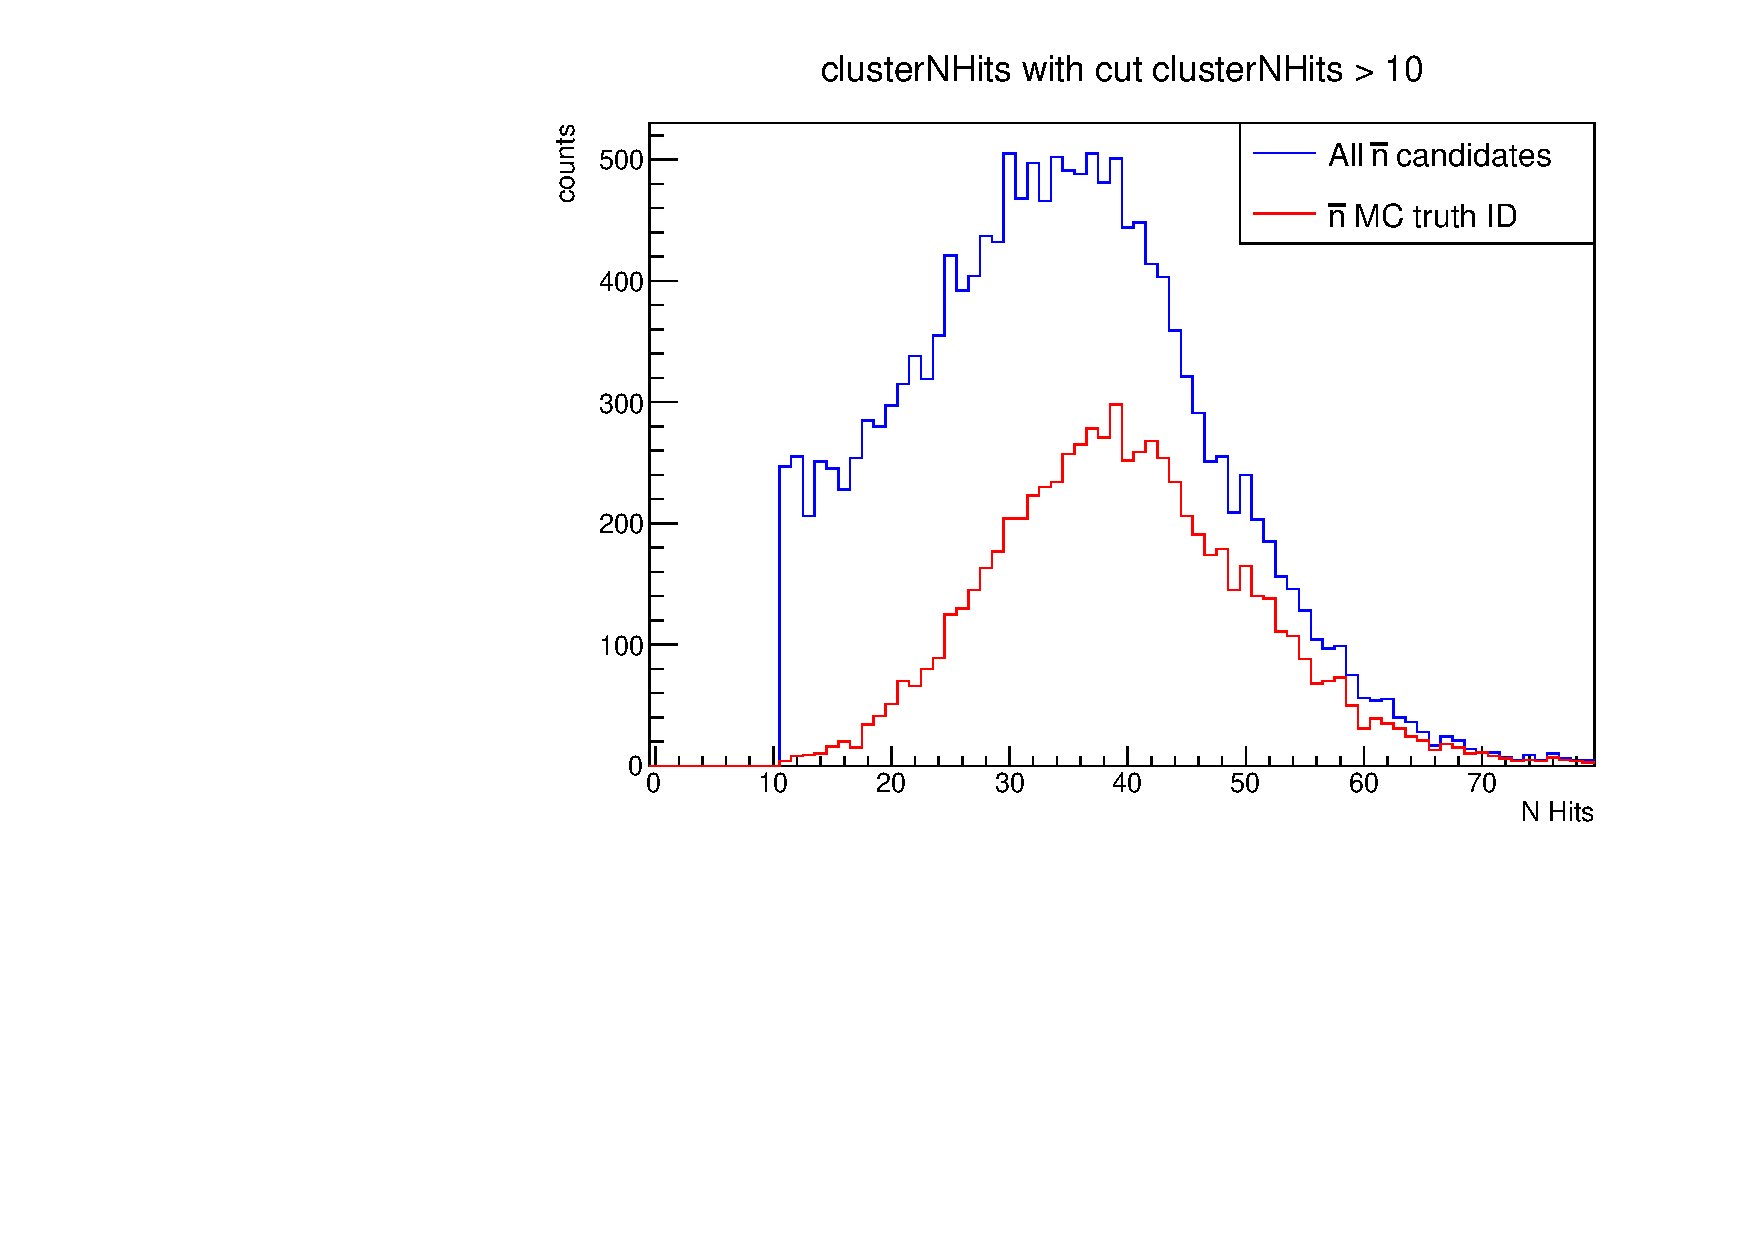
\includegraphics[width=0.49\textwidth]{nbar_MC/images/clusterNHits_hitscut_isr.pdf}
   
     \caption{Comparison of reconstructed cluster variables for all $\bar{n}$ candidates (blue) and those associated with $\bar{n}$ particles by Monte Carlo truth Monte Carlo PDG = -2112  (red) (ISR case). Cut $clusterNHits > 10$ is performed.}
     
     \label{fig:cluster_ISR_NHits}

\end{figure}
 \begin{figure}[h]
    \centering
    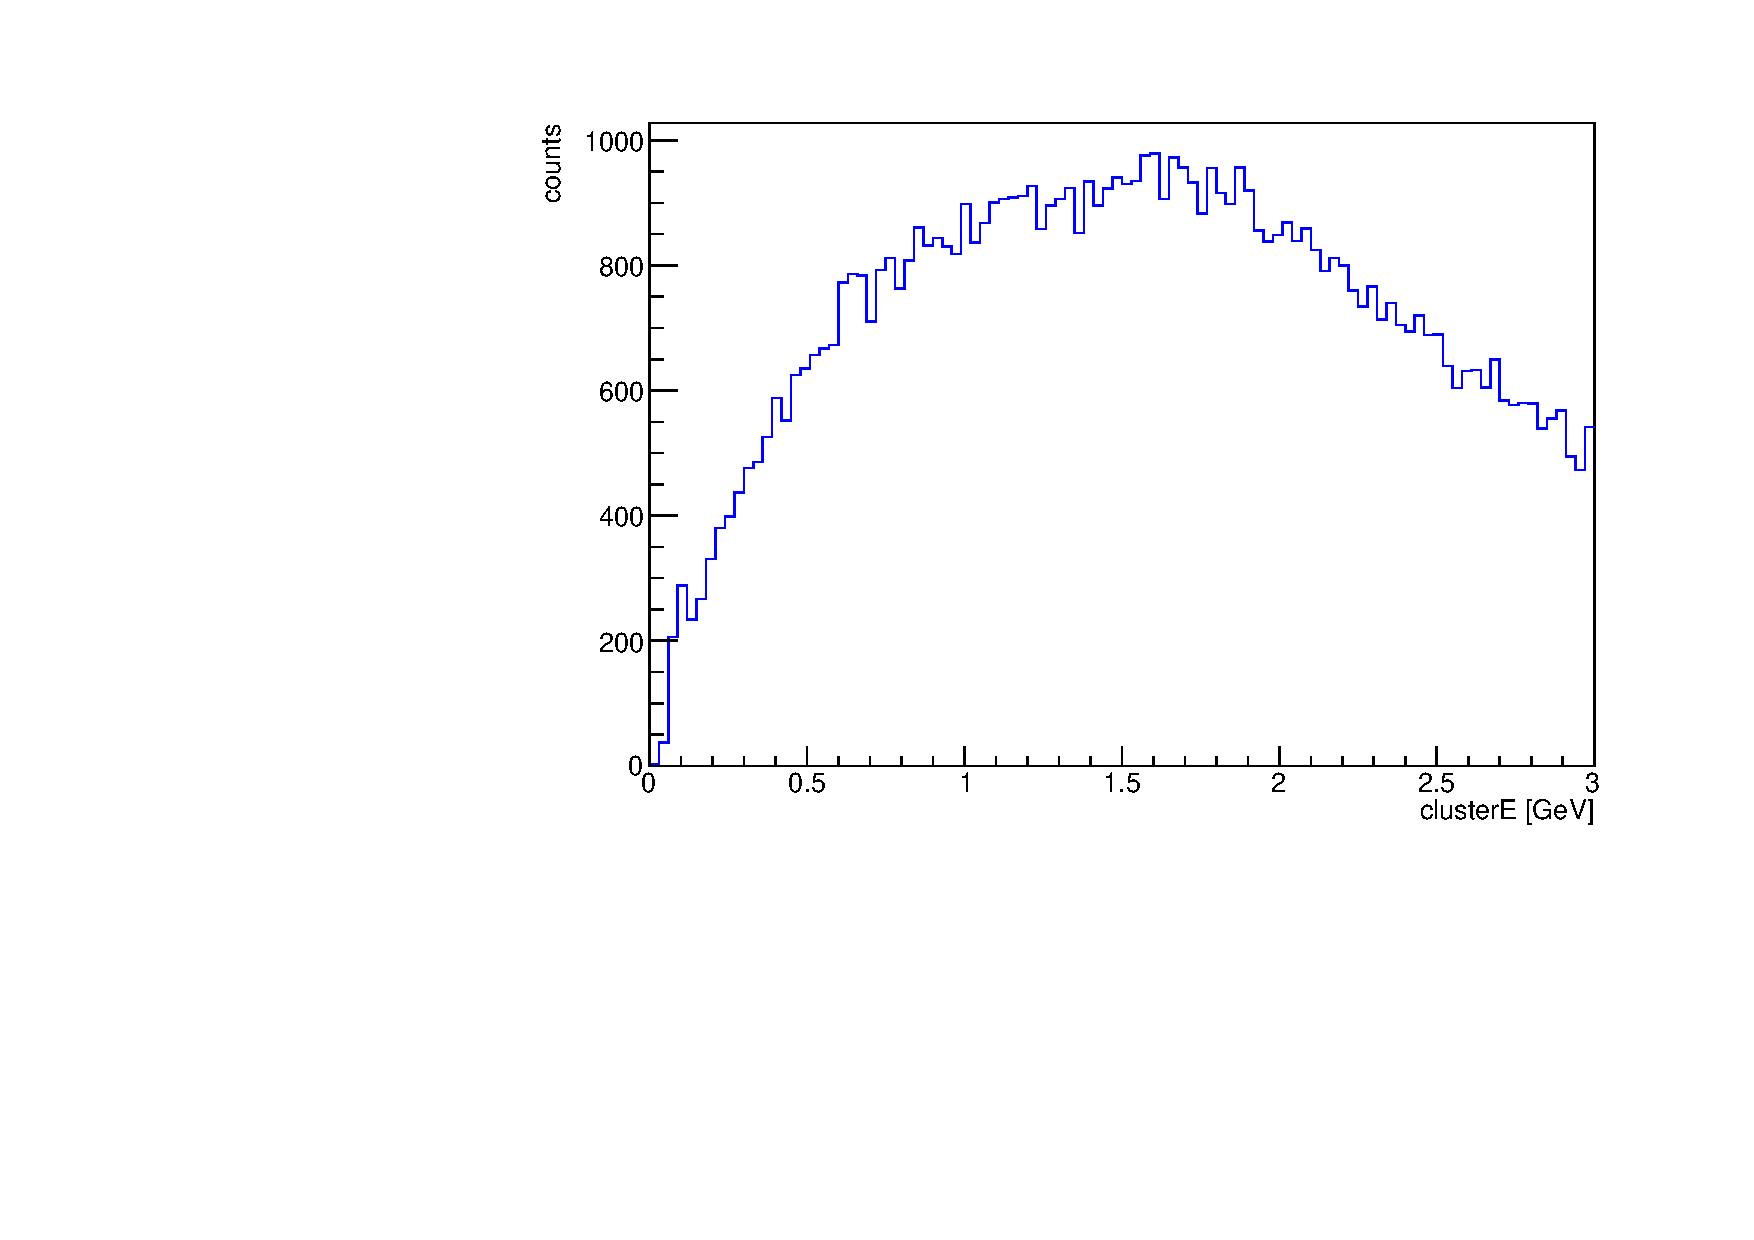
\includegraphics[width=0.49\textwidth]{nbar_cocktail/images/clusterE_isr_qqbar.pdf}
    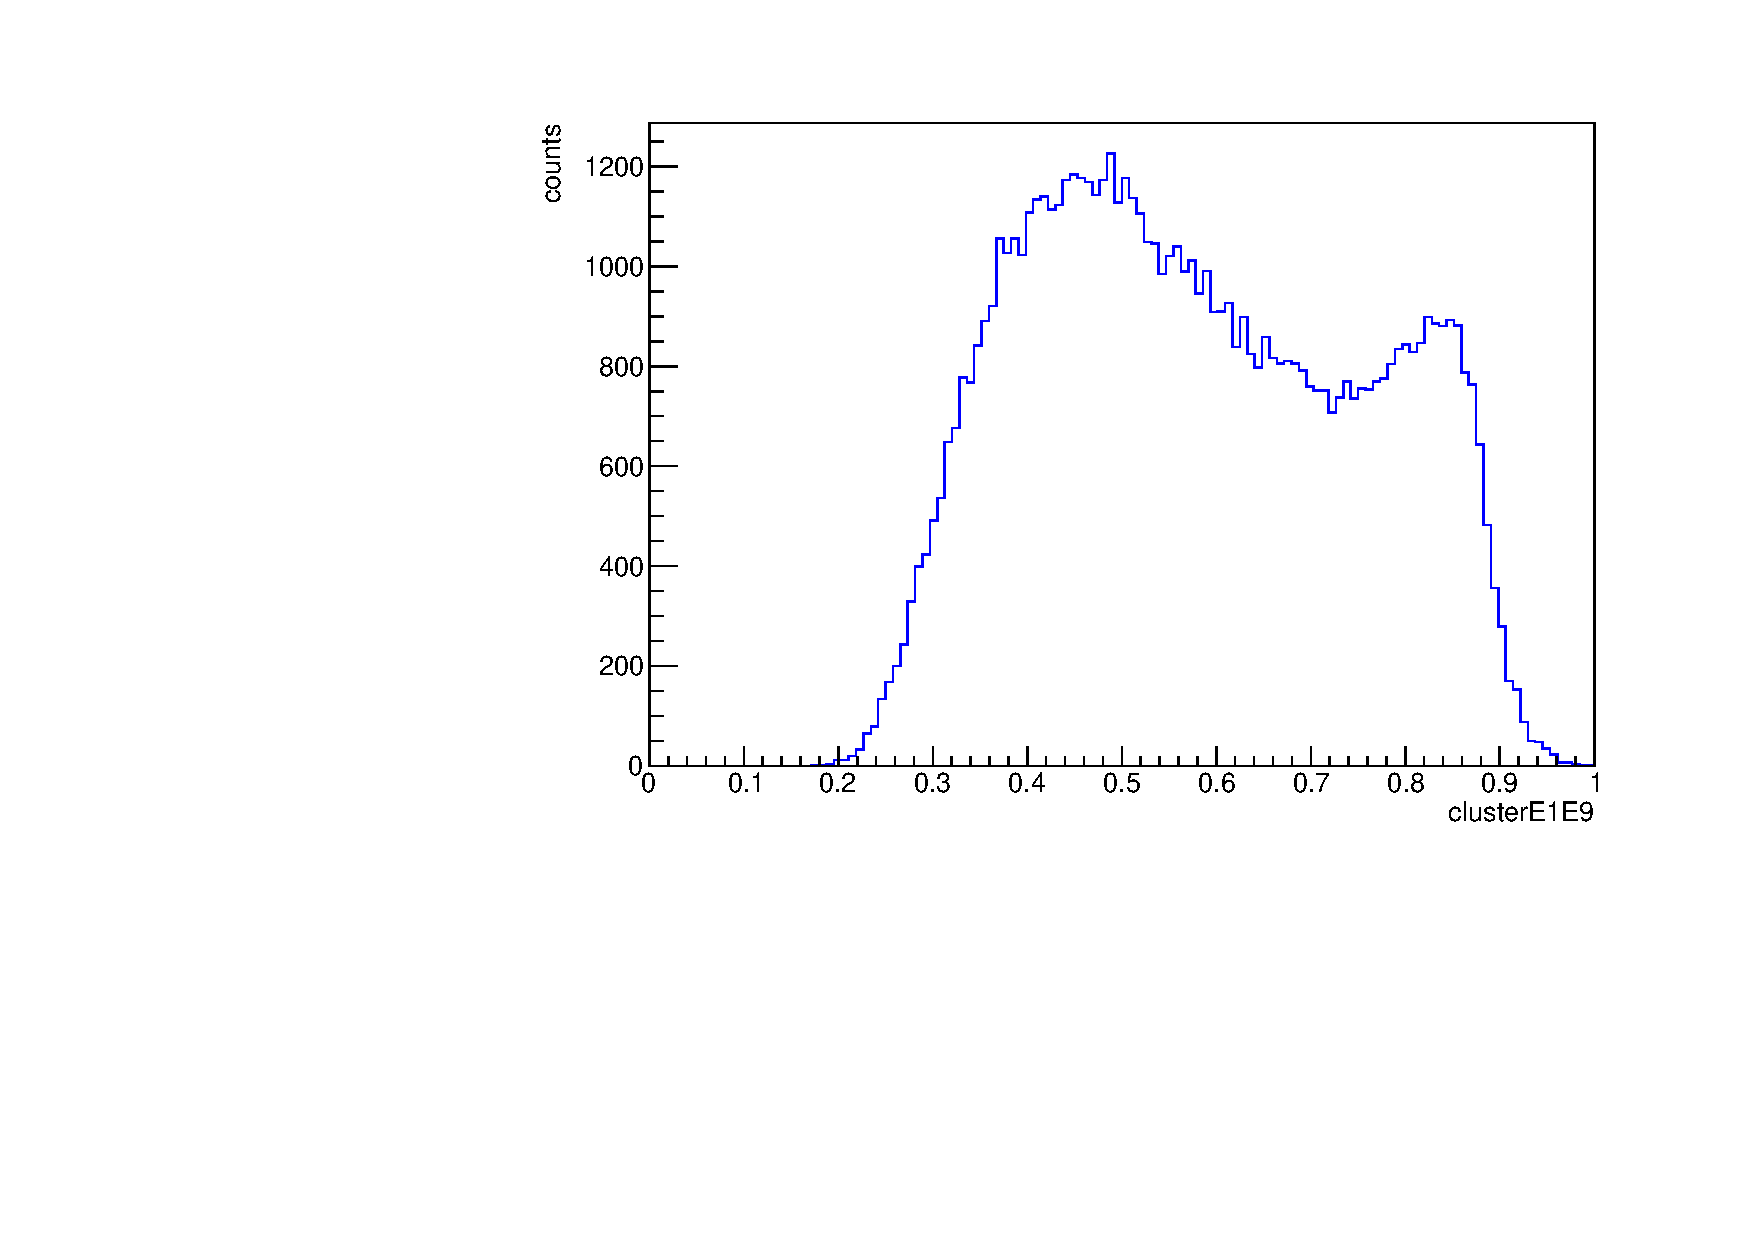
\includegraphics[width=0.49\textwidth]{nbar_cocktail/images/clusterE1E9_isr_qqbar.pdf}
    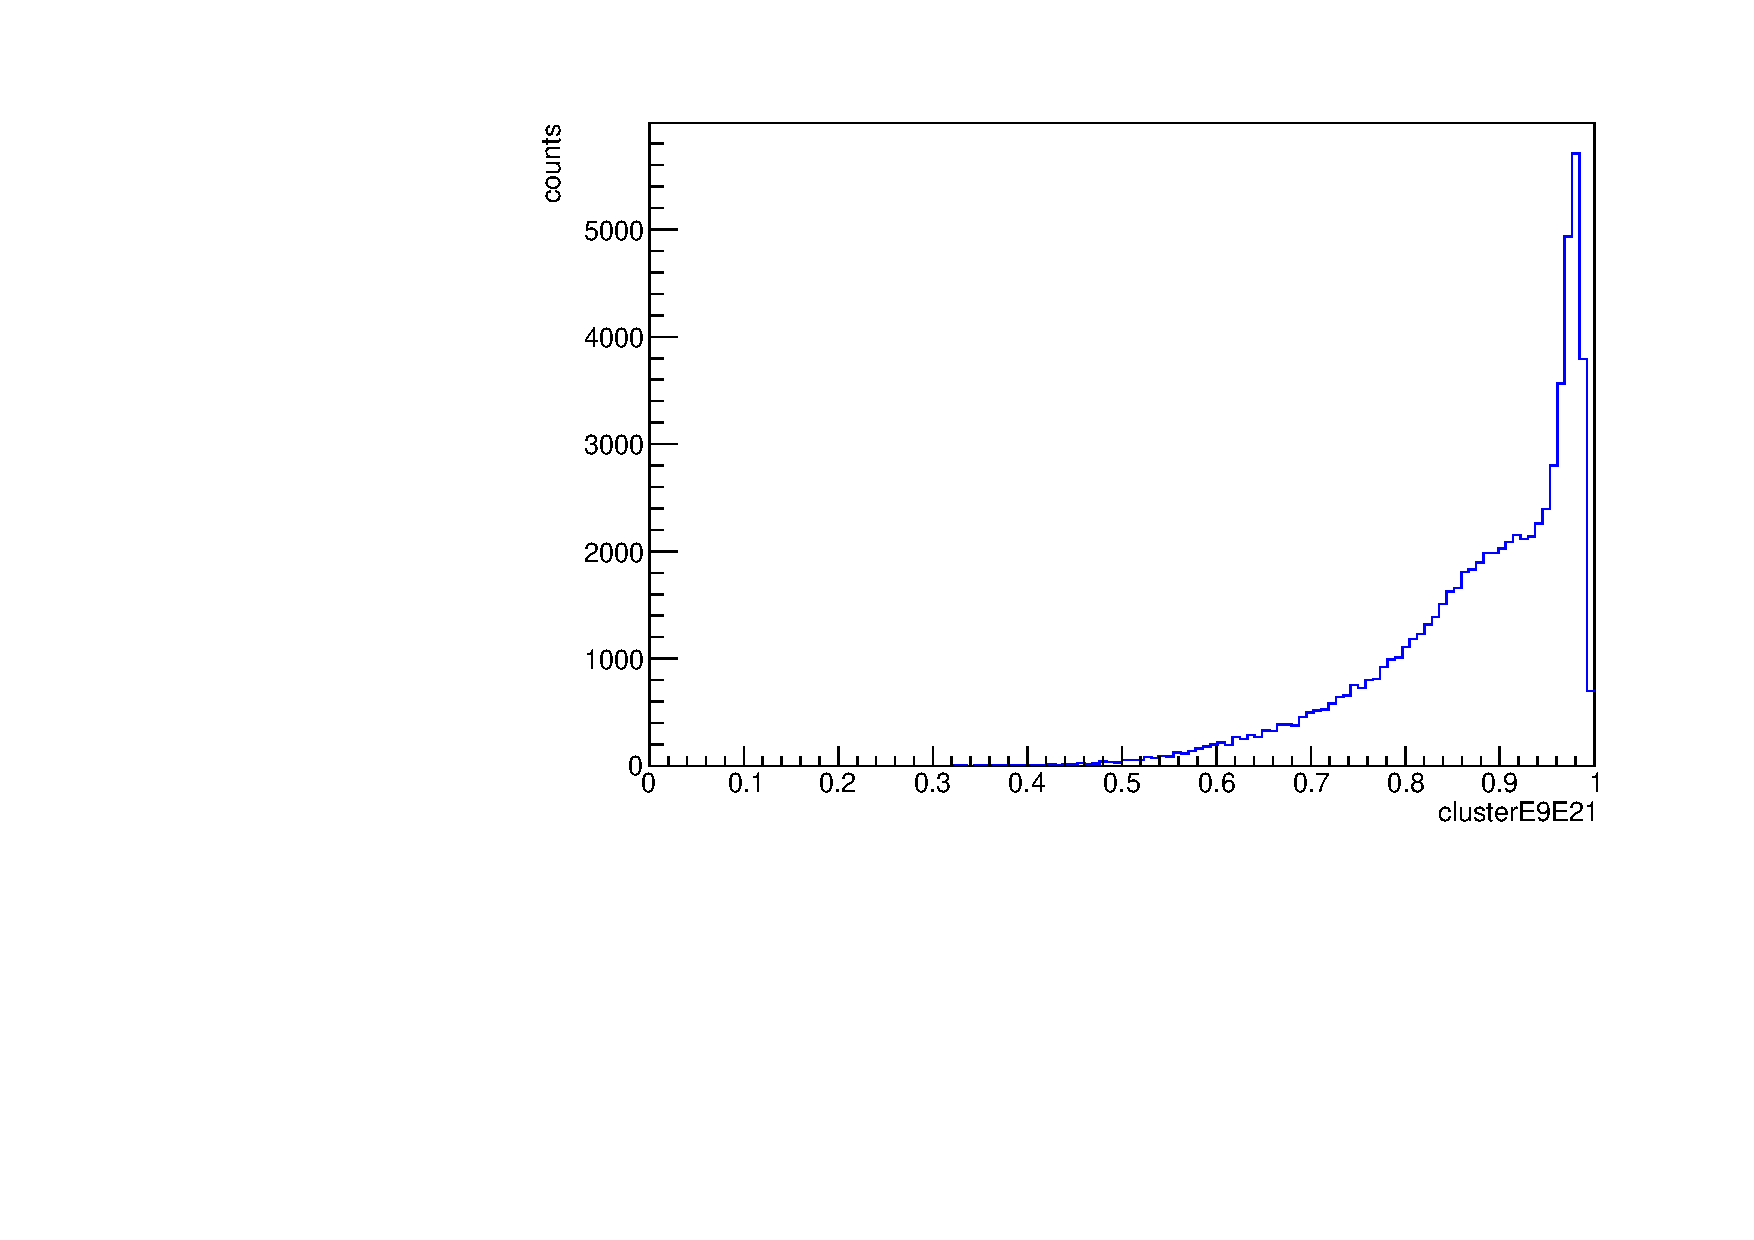
\includegraphics[width=0.49\textwidth]{nbar_cocktail/images/clusterE9E21_isr_qqbar.pdf}
    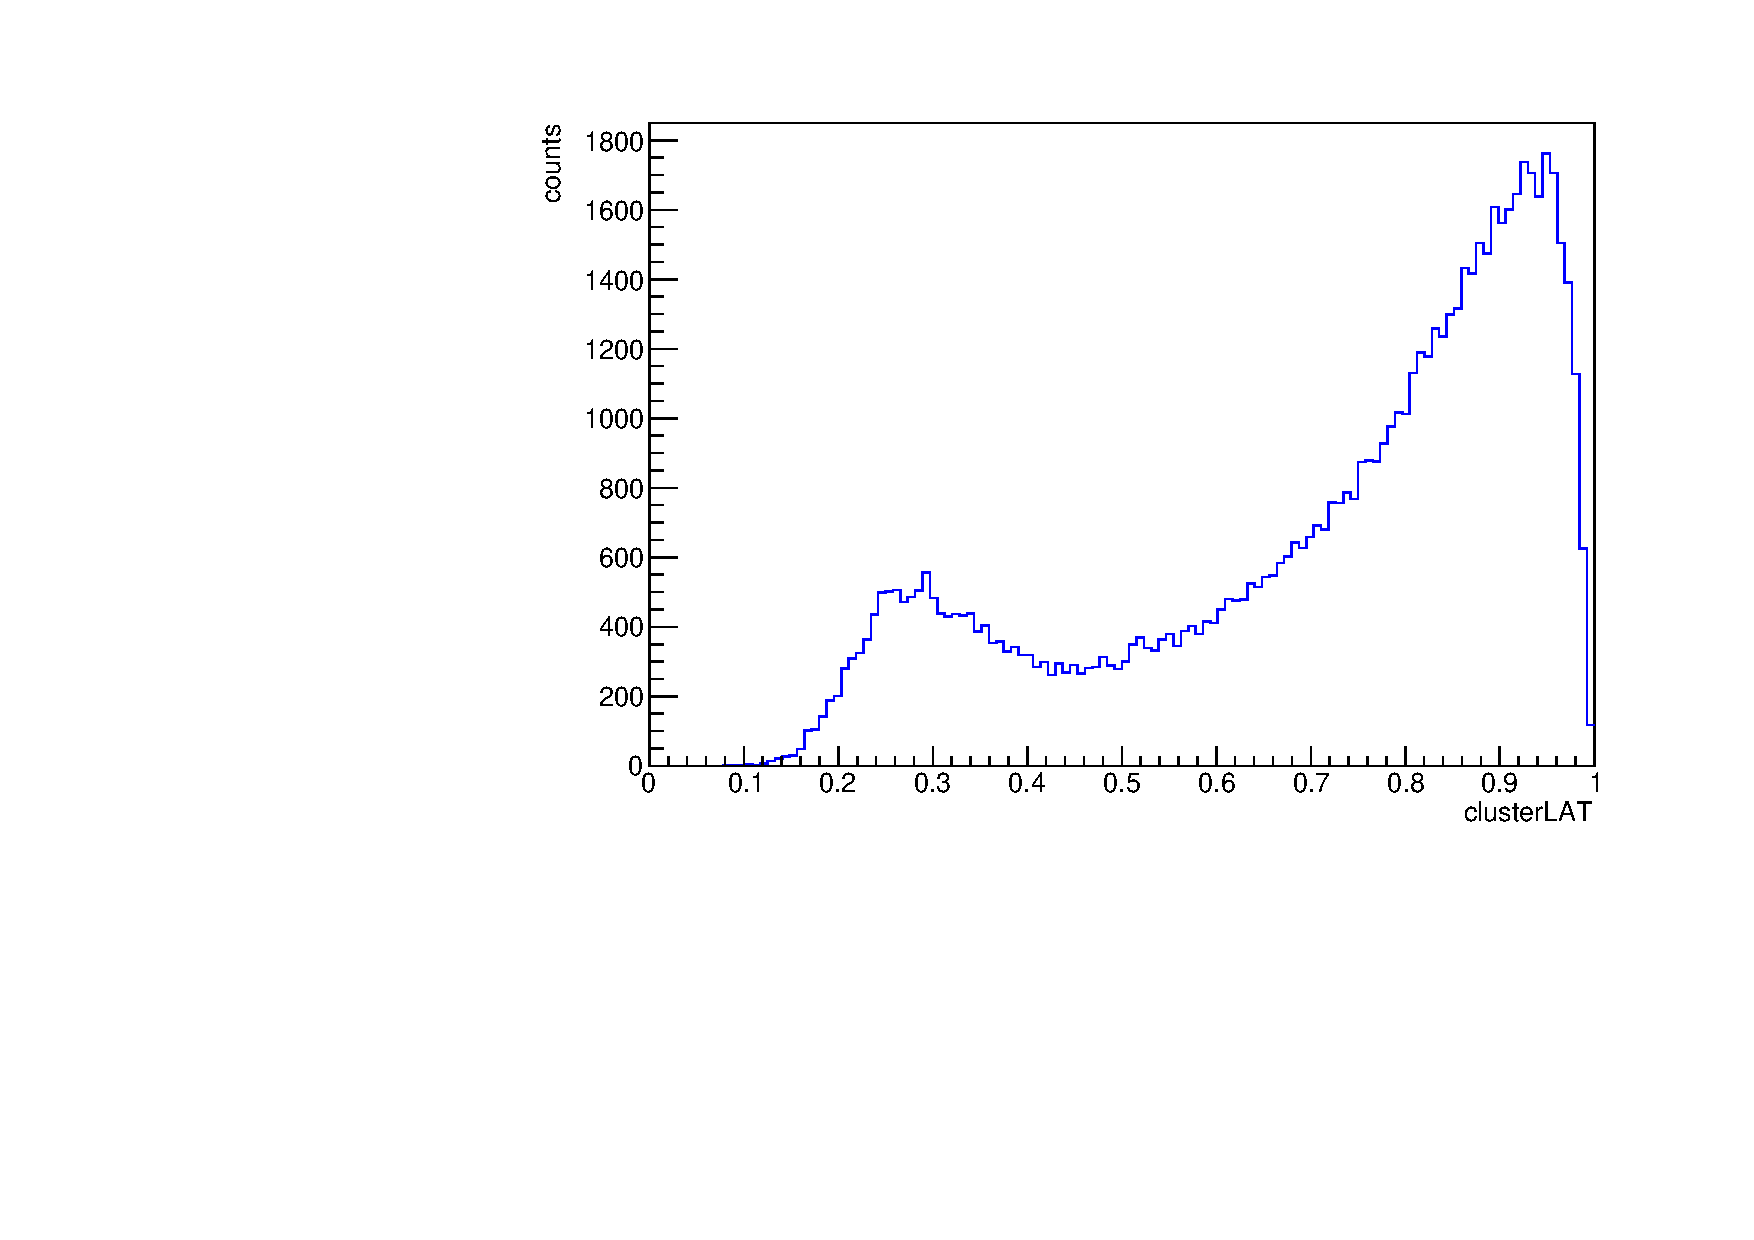
\includegraphics[width=0.49\textwidth]{nbar_cocktail/images/clusterLAT_isr_qqbar.pdf}
    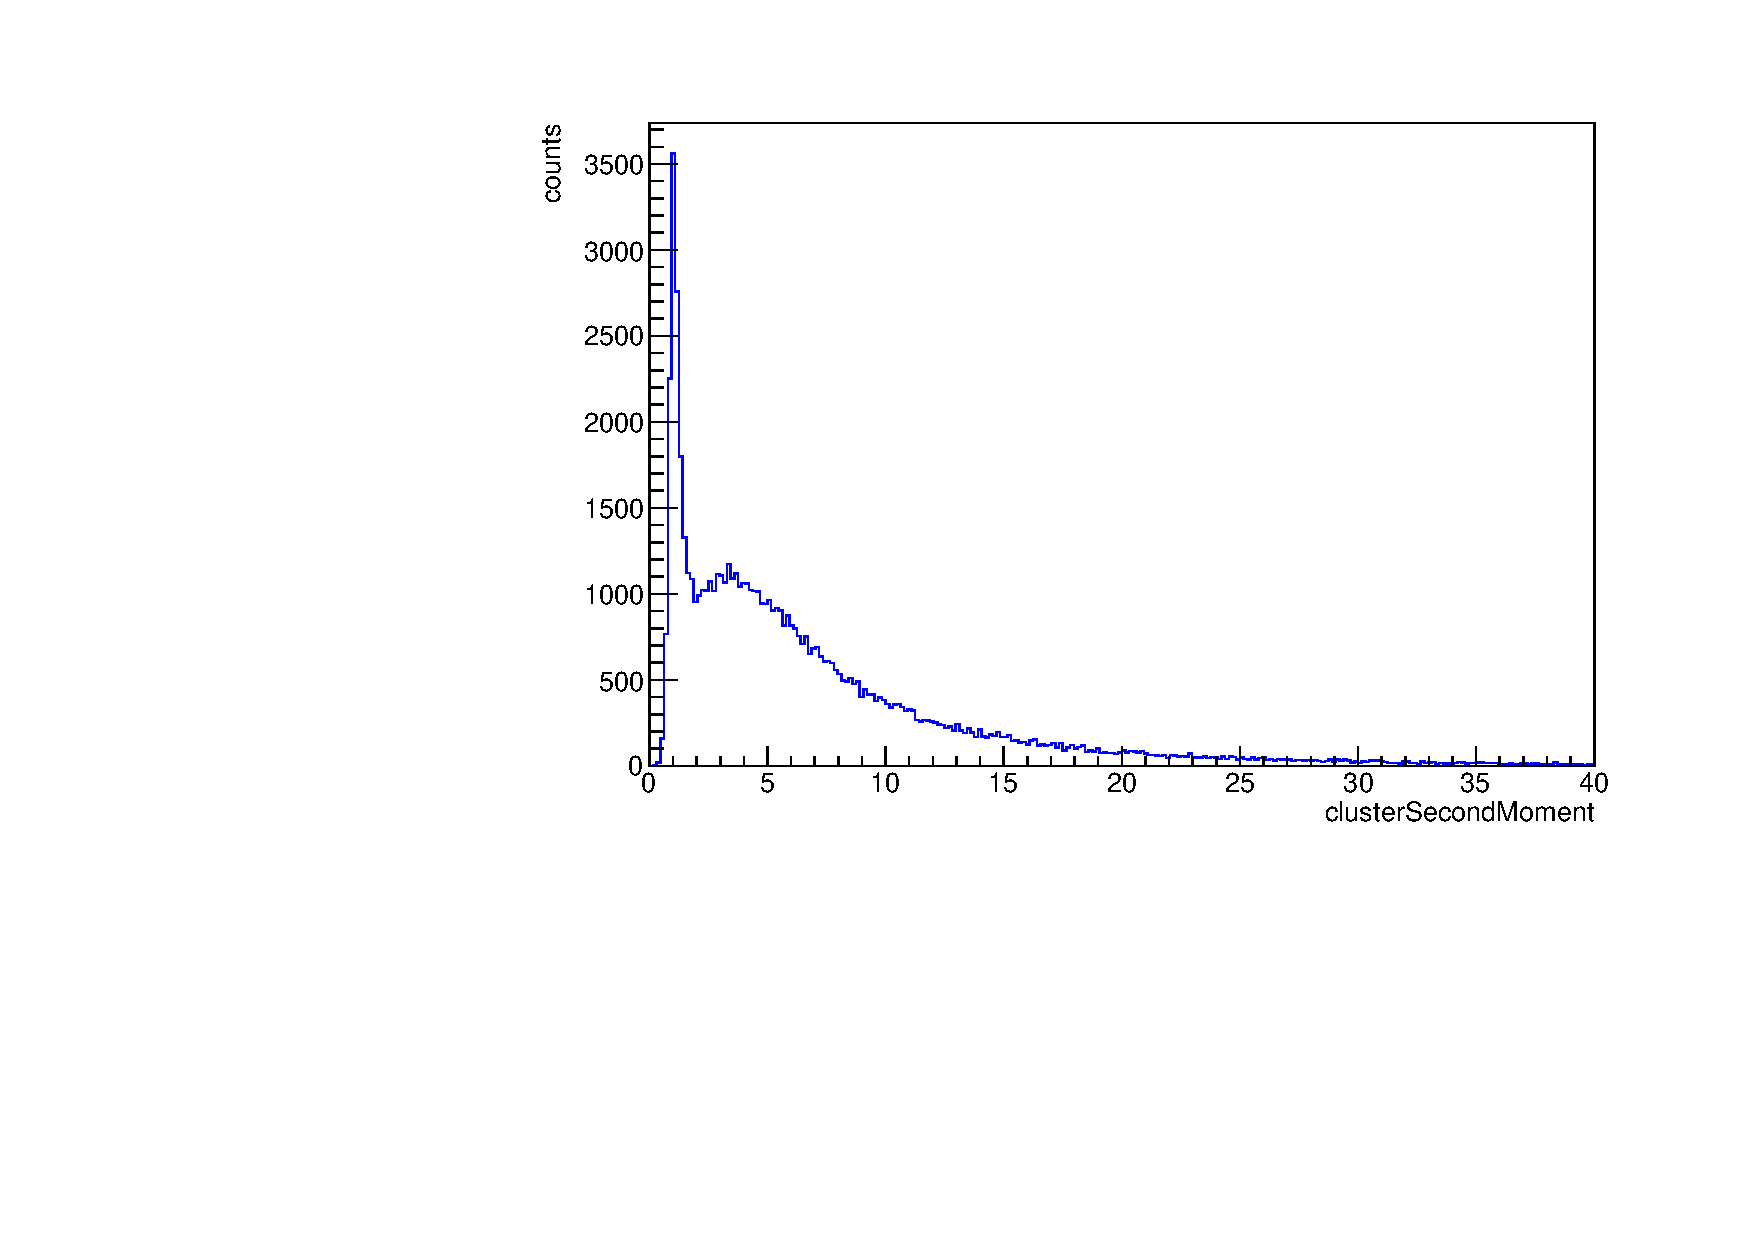
\includegraphics[width=0.49\textwidth]{nbar_cocktail/images/clusterSecondMoment_isr_qqbar.pdf}
    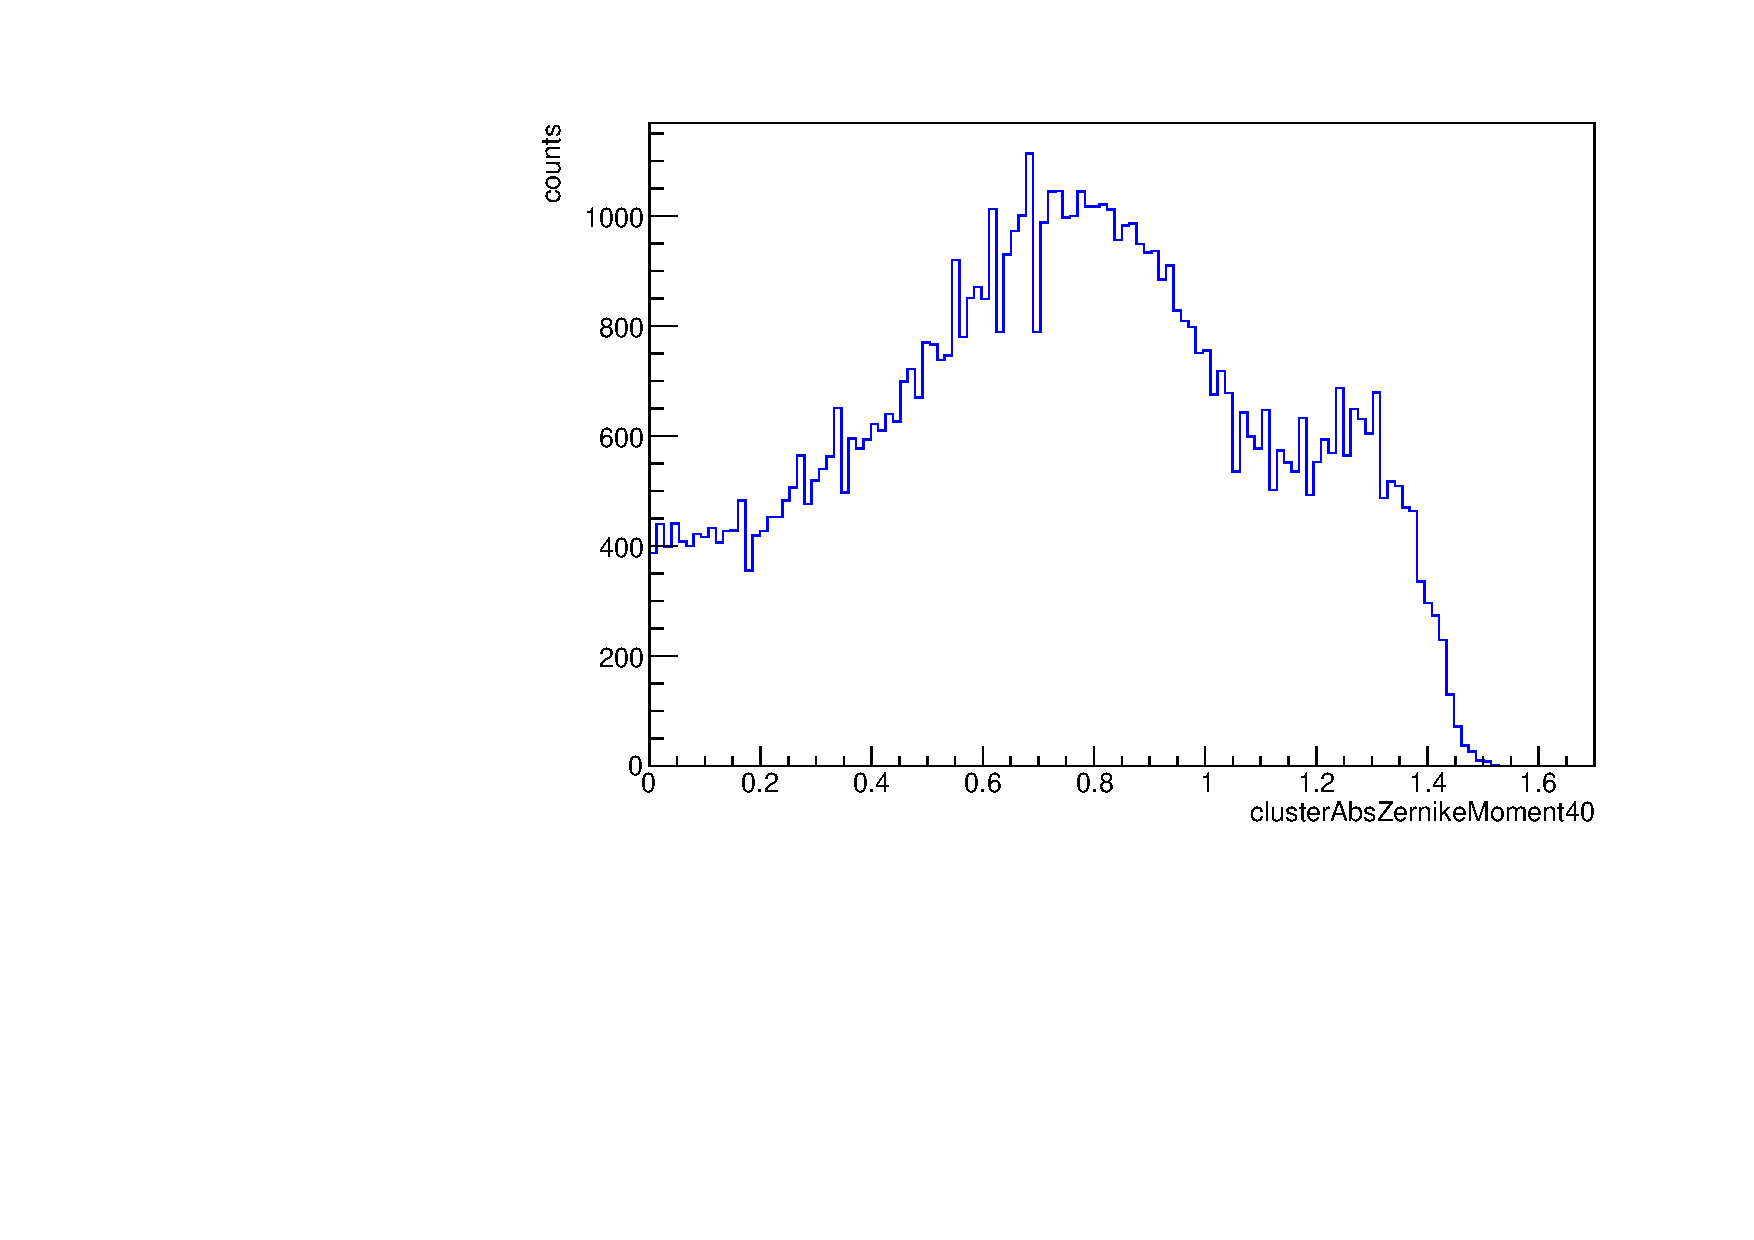
\includegraphics[width=0.49\textwidth]{nbar_cocktail/images/clusterAbsZernikeMoment40_isr_qqbar.pdf}
    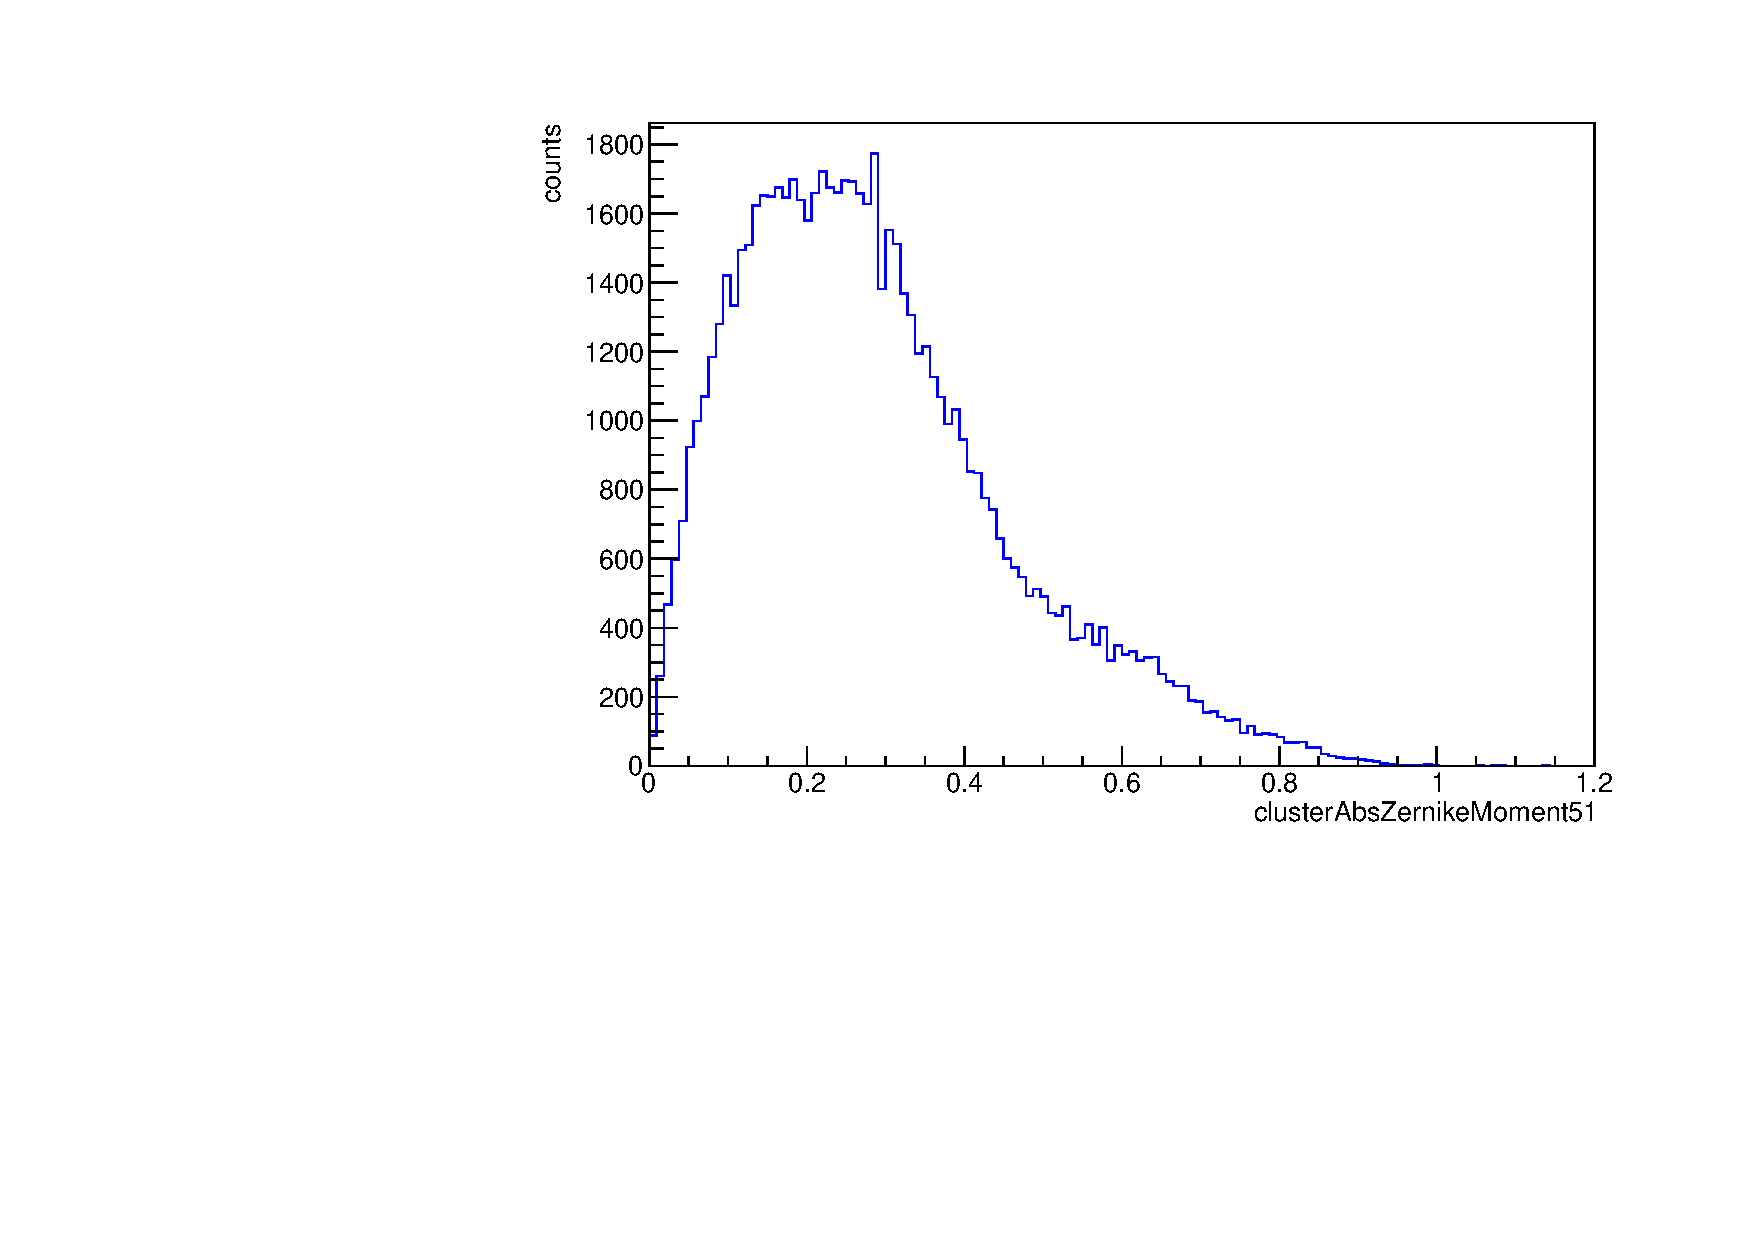
\includegraphics[width=0.49\textwidth]{nbar_cocktail/images/clusterAbsZernikeMoment51_isr_qqbar.pdf}
    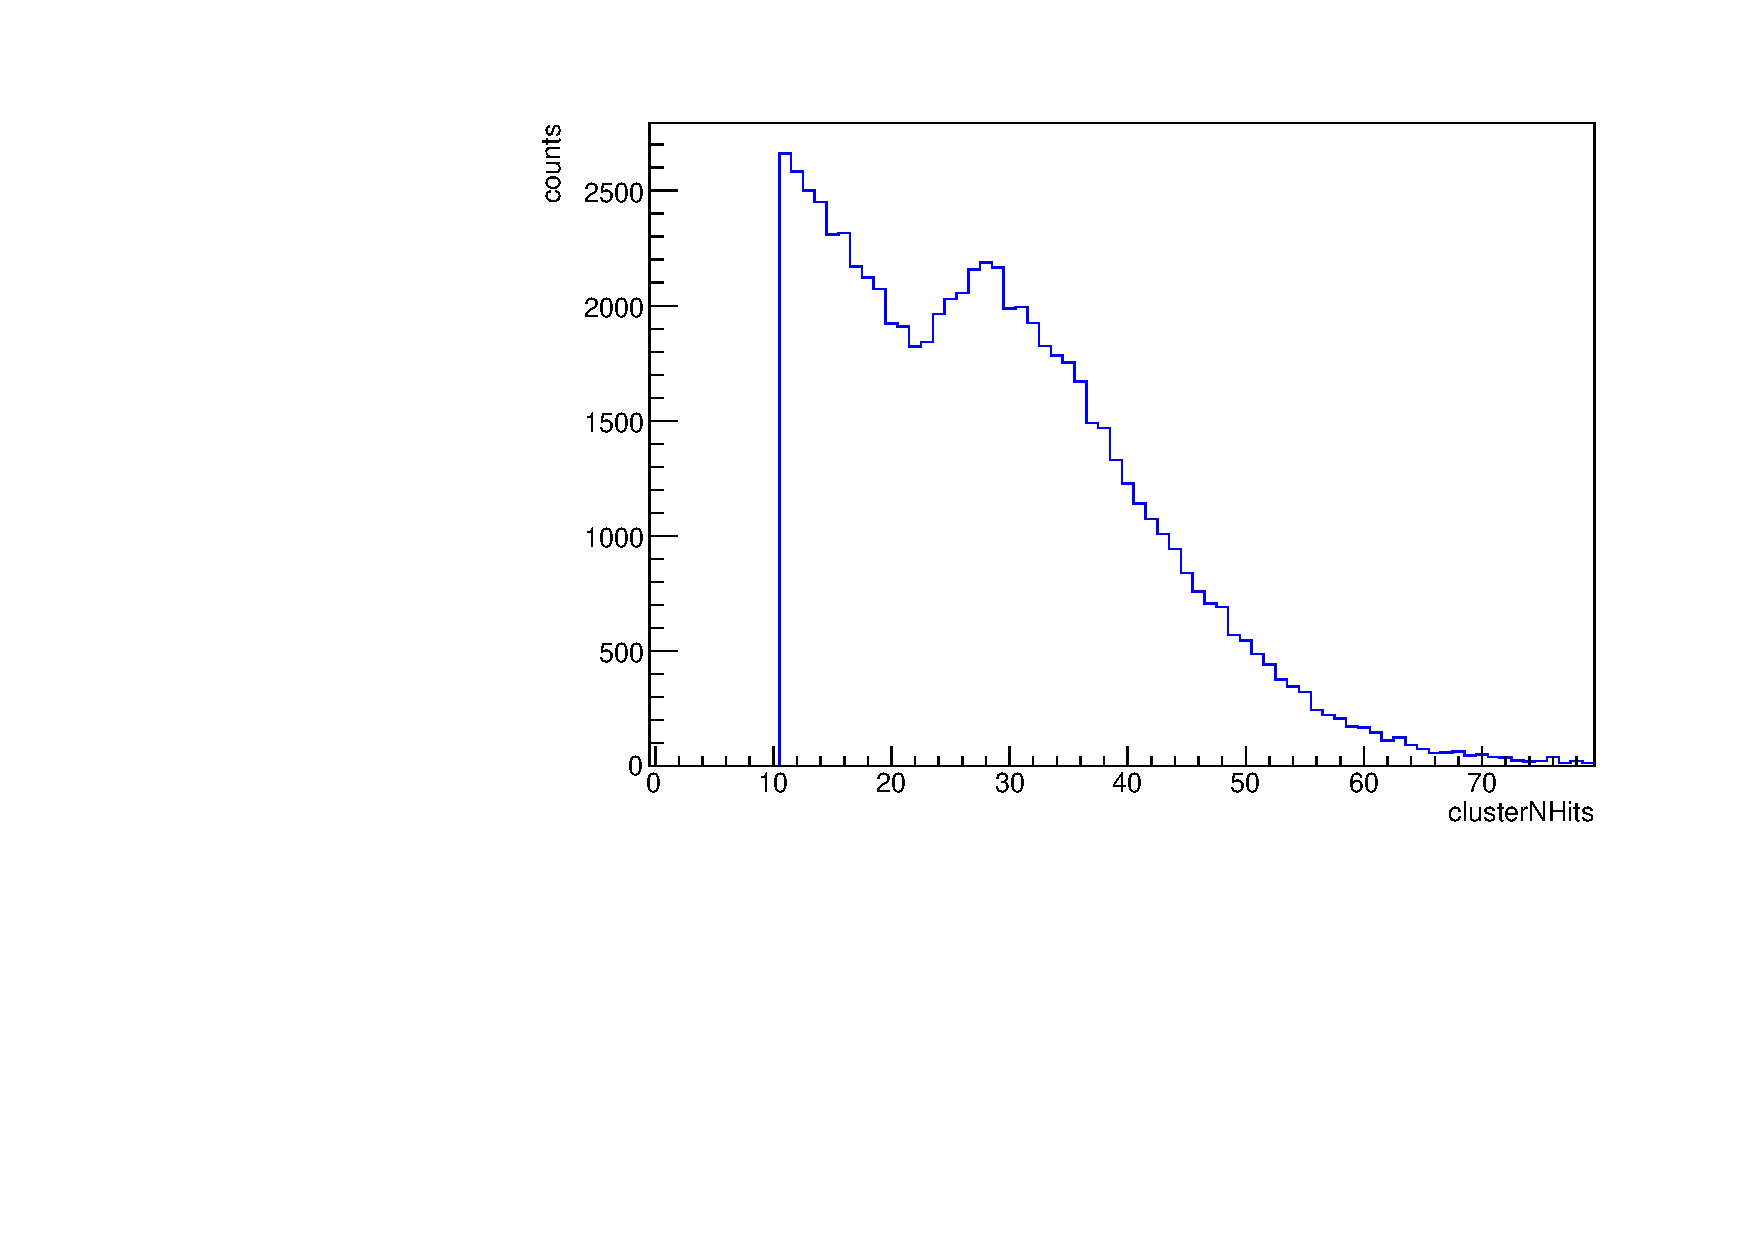
\includegraphics[width=0.49\textwidth]{nbar_cocktail/images/clusterNHits_isr_qqbar.pdf}
     \caption{Reconstructed cluster variables distribution for $\bar{n}$ candidates in the for the recoil mass region [0, 2] GeV$c^2$/, in ISR case. q$\bar{q}$ cocktail.}
     \label{fig:clus_vars_isr_qqbar}
\end{figure}
